% !TEX program = xelatex
% Git 与 VS Code 实战教程（全彩插图版）
% 使用 xelatex + ctex 编译

\documentclass[12pt,a4paper,openany]{ctexbook}

% ==================== 宏包 ====================
\usepackage[margin=2.5cm,headheight=15pt]{geometry}
\usepackage{graphicx}
\usepackage{xcolor}
\usepackage{listings}
\usepackage{booktabs}
\usepackage{longtable}
\usepackage{array}
\usepackage{enumitem}
\usepackage{tcolorbox}
\usepackage{fontawesome5}
\usepackage{hyperref}
\usepackage{tikz}
\usetikzlibrary{positioning}
\usepackage{fancyhdr}
\usepackage{titlesec}
\usepackage{tabularx}
\usepackage{multicol}
\usepackage{float}
\usepackage{caption}
\usepackage{wrapfig}

% colortbl 未安装时 \arrayrulecolor 无定义；提供 no-op 垫片保证兼容。
% （未加载 colortbl 时 booktabs 规则线默认即为黑色，功能等价于 \arrayrulecolor{black}）
\providecommand{\arrayrulecolor}[1]{}

% ==================== 颜色定义 ====================
\definecolor{gitorange}{RGB}{240,80,50}
\definecolor{gitdark}{RGB}{40,40,40}
\definecolor{codebg}{RGB}{248,248,248}
\definecolor{codeframe}{RGB}{200,200,200}
\definecolor{tipgreen}{RGB}{46,125,50}
\definecolor{warnred}{RGB}{198,40,40}
\definecolor{infoblue}{RGB}{21,101,192}
\definecolor{sectioncolor}{RGB}{33,33,33}
\definecolor{linkcolor}{RGB}{25,118,210}
\definecolor{imgborder}{RGB}{180,180,180}

% ==================== 超链接设置 ====================
\hypersetup{
  colorlinks=true,
  linkcolor=linkcolor,
  urlcolor=linkcolor,
  citecolor=linkcolor,
  bookmarksnumbered=true,
  pdfstartview=FitH
}

% ==================== 代码列表设置 ====================
\lstset{
  basicstyle=\ttfamily\small,
  backgroundcolor=\color{codebg},
  frame=single,
  rulecolor=\color{codeframe},
  breaklines=true,
  breakatwhitespace=false,
  breakautoindent=true,
  columns=flexible,
  keepspaces=true,
  showstringspaces=false,
  tabsize=2,
  keywordstyle=\color{gitorange}\bfseries,
  commentstyle=\color{gray}\itshape,
  stringstyle=\color{tipgreen},
  morekeywords={git,github,gh},
  literate=
    {┌}{{\textbar}}1 {┐}{{\textbar}}1
    {└}{{\textbar}}1 {┘}{{\textbar}}1
    {│}{{\textbar}}1 {─}{{-}}1
}

\lstdefinestyle{shell}{
  basicstyle=\ttfamily\small,
  backgroundcolor=\color{codebg},
  frame=single,
  rulecolor=\color{codeframe},
  breaklines=true,
  columns=flexible,
  keepspaces=true,
  showstringspaces=false,
  moredelim=[il][\color{gray}]{\#},
}
\lstdefinestyle{shellinbox}{basicstyle=\ttfamily\small, frame=none, backgroundcolor={}, breaklines=true, columns=flexible, keepspaces=true, showstringspaces=false, moredelim=[il][\color{gray}]{\#}, xleftmargin=0pt, xrightmargin=0pt, aboveskip=0pt, belowskip=0pt, framesep=0pt}

% ==================== 提示框定义 ====================
\tcbuselibrary{skins,breakable}

\newenvironment{tipbox}{%
  \medskip
  \noindent\textbf{\faLightbulb\; 提示}
  \smallskip
}{%
  \medskip
}

\newtcolorbox{warnbox}[1][]{
  colback=white,
  colframe=warnred,
  fonttitle=\bfseries,
  title={\faExclamationTriangle\; 注意},
  breakable,
  #1
}

\newtcolorbox{infobox}[1][]{
  colback=white,
  colframe=infoblue,
  fonttitle=\bfseries,
  title={\faInfoCircle\; 说明},
  breakable,
  #1
}

\newenvironment{keybox}{%
  \medskip
  \noindent\textbf{\faKey\; 核心概念}
  \smallskip
}{%
  \medskip
}

\newenvironment{stepbox}{%
  \medskip
  \noindent\textbf{\faCogs\; 操作步骤}
  \smallskip
}{%
  \medskip
}
\renewcommand{\figurename}{图}
\renewcommand{\tablename}{表}

% ==================== 图片包装命令 ====================
\newcommand{\vscodeimg}[3]{%
  \begin{figure}[H]
    \centering
    \fcolorbox{imgborder}{white}{\includegraphics[width=0.92\textwidth]{#1}}
    \caption{#2}\label{#3}
  \end{figure}
}

\newcommand{\vscodeimgnarrow}[3]{%
  \begin{figure}[H]
    \centering
    \fcolorbox{imgborder}{white}{\includegraphics[width=0.72\textwidth]{#1}}
    \caption{#2}\label{#3}
  \end{figure}
}

\newcommand{\vscodeimgwide}[3]{%
  \begin{figure}[H]
    \centering
    \fcolorbox{imgborder}{white}{\includegraphics[width=\textwidth]{#1}}
    \caption{#2}\label{#3}
  \end{figure}
}

% ==================== 页眉页脚 ====================
\pagestyle{fancy}
\fancyhf{}
\fancyhead[LE,RO]{\thepage}
\fancyhead[LO]{\nouppercase{\rightmark}}
\fancyhead[RE]{\nouppercase{\leftmark}}
\renewcommand{\headrulewidth}{0.4pt}

% ==================== 章节标题样式 ====================
\titleformat{\chapter}[display]
  {\normalfont\Huge\bfseries\color{sectioncolor}}
  {\chaptertitlename\ \thechapter}{20pt}{\Huge}
  [\vspace{2ex}{\titlerule}]

\titleformat{\section}
  {\normalfont\Large\bfseries\color{gitdark}}
  {\thesection}{1em}{}
  [\vspace{0.5ex}{\titlerule[0.3pt]}]

% ==================== 文档信息 ====================
\title{%
  \vspace{-2cm}
  {\Huge\bfseries Git 与 VS Code 实战教程}\\[0.5cm]
  {\LARGE 从入门到精通的完整指南}\\[1cm]
  {\large 涵盖 Git 核心概念、GitHub 协作与 VS Code 深度集成}\\[0.3cm]
  {\normalsize\color{gray} 全彩插图版 · 含 27 张 VS Code 真实界面截图}
}
\author{}
\date{\today}

% ==================== 正文开始 ====================
\begin{document}

% ---------- 封面 ----------
\maketitle
\thispagestyle{empty}

\vspace{2cm}
\begin{center}
\begin{tcolorbox}[
  colback=gray!5!white,
  colframe=gray!50!black,
  title={\faBook\; 关于本文档},
  fonttitle=\bfseries\large
]
本文档是一份面向初学者的 Git 与 GitHub 完整教程，重点讲解如何在 Visual Studio Code（VS Code）
中利用 Git 进行高效的代码版本管理。

\textbf{本版本特色}：
\begin{itemize}
  \item 全文包含 \textbf{27 张} VS Code 真实界面截图，每个操作都有对应的界面演示
  \item 从概念到实操，图文并茂，降低学习门槛
  \item 同时覆盖命令行和 VS Code 图形界面两种操作方式
\end{itemize}

\vspace{0.5em}
\textbf{适用对象}：编程初学者、希望学习版本控制的开发者、希望从命令行迁移到图形化工作流的 Git 用户。

\vspace{0.5em}
\textbf{前置要求}：基本的计算机操作能力；已安装或准备安装 Git 和 VS Code。
\end{tcolorbox}
\end{center}

\clearpage

% ---------- 目录 ----------
\tableofcontents
\clearpage

% ================================================================
%  第 0 章：开始前的准备——建立心智模型
% ================================================================
\chapter*{第 0 章：开始前的准备——建立心智模型}
\addcontentsline{toc}{chapter}{第 0 章：开始前的准备——建立心智模型}

\markboth{第 0 章：开始前的准备}{第 0 章：开始前的准备}

如果你完全没接触过 Git、GitHub、版本控制，请先花 5 分钟读完这一章。
不需要记命令，只要建立三个**生活类比**，后面学起来就会顺畅很多。

\begin{warnbox}
\textbf{为什么需要版本控制？}

想象一下这样的场景：你正在写一个网站项目，代码文件名叫 \texttt{index.html}。你改了一版，觉得不太对，于是复制了一份，命名为 \texttt{index\_v2.html}；又改了一版，变成 \texttt{index\_v3\_final.html}；后来又发现有个 bug，于是有了 \texttt{index\_v3\_final\_真的.html}……一周以后，你的文件夹里堆满了各种版本的文件，你已经完全忘记哪个才是"最终版"。

这还只是一个人工作的场景。如果团队里三个人同时修改同一个文件呢？你改完传给同事，同事改完传回来，你再改——文件名变成了 \texttt{index\_张三\_改.html}、\texttt{index\_李四\_改\_最终.html}。最后，你们都不知道该用哪个版本了。

版本控制系统就是为解决这些问题而生的。它自动记录每一次修改，让你可以随时回到过去的任意版本，还能让多人协作时不再"文件满天飞"。
\end{warnbox}

\section{三个核心类比}

三者关系如图~\ref{fig:three-analogies} 所示——
\begin{figure}[H]\centering
\begin{tikzpicture}[
  box/.style={draw, rounded corners=10pt, minimum width=3.5cm, minimum height=3.5cm,
              font=\small, align=center, text width=4cm, fill=#1, inner sep=8pt},
  arr/.style={->, thick, >=stealth},
  node distance=2.5cm
]
  \node[box=blue!15] (git) at (0,0) {
    \textbf{Git = 时光机}\\
    \faClock~ 记录每一次修改\\
    \faUndo~ 可随时回到过去版本\\
    \faCodeBranch~ 可在平行宇宙开发新功能
  };
  \node[box=green!15] (github) at (7,0) {
    \textbf{GitHub = 云端仓库}\\
    \faCloud~ 代码存在云上\\
    \faUsers~ 多人协作的中心枢纽\\
    \faGlobe~ 换电脑也能接着干
  };
  \node[box=orange!15] (vscode) at (3.5,-5.5) {
    \textbf{VS Code = 驾驶舱}\\
    \faMousePointer~ 点按钮代替敲命令\\
    \faEye~ 可视化看变更、冲突、历史\\
    \faMagic~ AI 帮写提交信息
  };

  \draw[arr] (git) -- node[above, font=\small, align=center]{推送/拉取} (github);
  \draw[arr] (vscode) -- node[left, font=\small, align=center]{图形化操作} (git);
  \draw[arr] (vscode) -- node[right, font=\small, align=center]{一键同步} (github);
\end{tikzpicture}
\caption{Git、GitHub 与 VS Code 的关系——三者协作构成完整的版本控制工作流}\label{fig:three-analogies}\end{figure}

\subsection{Git 是「时光机」}

\begin{itemize}[leftmargin=2em]
  \item \textbf{写代码 = 穿越时空}：每次 \texttt{git commit} 就是按下「存档」，生成一个唯一的「存档编号」（哈希值）。
  \item \textbf{想回去 = 时光倒流}：\texttt{git restore} / \texttt{git reset} 让你回到任意一次存档的瞬间。
  \item \textbf{想尝试新想法 = 进入平行宇宙}：\texttt{git switch -c 新分支} 创建一个互不干扰的平行世界，搞砸了删掉分支就行，主世界毫发无损。
\end{itemize}

\begin{tipbox}
\textbf{零基础心法}：别怕弄坏！Git 设计的初衷就是让你「大胆试错，随时后悔」。
\end{tipbox}

\subsection{GitHub 是「云端仓库」}

\begin{itemize}[leftmargin=2em]
  \item \textbf{备份}：电脑丢了、硬盘坏了，代码在 GitHub 上还在。
  \item \textbf{协作}：同事把代码传上来，你拉下来，合在一起，不用 U 盘传文件。
  \item \textbf{展示}：开源项目放在 GitHub，全世界都能看、能用、能提改进建议。
\end{itemize}

\subsection{VS Code 是「驾驶舱」}

\begin{itemize}[leftmargin=2em]
  \item 不用背命令：侧边栏点点鼠标，暂存、提交、推送、拉取、解决冲突全搞定。
  \item 所见即所得：文件旁边的颜色竖线（绿=新增、蓝=修改、红=删除）实时告诉你改了啥。
  \item AI 助手：点「魔法棒」自动生成提交信息，遇到冲突 AI 也能帮忙分析。
\end{itemize}

\section{本教程的学习路径图}

完整路径如图~\ref{fig:learning-path} 所示——
\begin{figure}[H]\centering
\resizebox{\textwidth}{!}{%
\begin{tikzpicture}[
  phase/.style={draw, rounded corners=8pt, minimum width=3.5cm, minimum height=1.6cm,
                font=\small\bfseries, align=center, text width=3cm, fill=#1},
  arr/.style={->, thick, >=stealth},
  node distance=1.8cm
]
  \node[phase=blue!20] (p0) at (0,0) {第 0 章\\建立心智模型\\\normalfont\small(5 分钟)};
  \node[phase=green!20] (p1) at (4,0) {第 1--3 章\\核心概念 + 基础操作\\\normalfont\small(2--3 小时)};
  \node[phase=yellow!20] (p2) at (8,0) {第 4--5 章\\分支协作 + 远程同步\\\normalfont\small(2--3 小时)};
  \node[phase=orange!20] (p3) at (12,0) {第 6--7 章\\VS Code 实战 + 完整流程\\\normalfont\small(1--2 小时)};
  \node[phase=red!20] (p4) at (6,-3) {附录\\避坑指南 + 命令速查\\\normalfont\small(随时查阅)};

  \draw[arr] (p0) -- (p1);
  \draw[arr] (p1) -- (p2);
  \draw[arr] (p2) -- (p3);
  \draw[arr] (p1) -- (p4);
  \draw[arr] (p2) -- (p4);
  \draw[arr] (p3) -- (p4);
\end{tikzpicture}
}
\caption{本教程学习路径——从心智模型到实战工作流的章节安排}\label{fig:learning-path}\end{figure}

\begin{infobox}
\textbf{建议阅读策略}：
\begin{itemize}
  \item \textbf{极速上手（30 分钟）}：只看第 0 章 $\to$ 第 1 章 1.1/1.2/1.5 $\to$ 第 2 章 2.1/2.2 $\to$ 第 3 章 3.1/3.4/3.5 $\to$ 第 7 章 7.2（VS Code 操作流）
  \item \textbf{系统掌握（1 周）}：按章节顺序完整阅读，每章做完「动手实验」再进入下一章
  \item \textbf{遇到问题查阅}：直接翻「附录：避坑指南」或「命令速查表」
\end{itemize}
\end{infobox}

\section{动手实验 0：验证环境就绪}

\medskip
\begin{enumerate}[leftmargin=1.5em]
  \item 打开终端（Windows 用 PowerShell，Mac/Linux 用 Terminal）
  \item 输入 \texttt{git --version}，看到版本号即表示 Git 已安装
  \item 输入 \texttt{code --version}，看到版本号即表示 VS Code 已安装且已加入 PATH
  \item 打开 VS Code，按 \texttt{Ctrl+Shift+G} 打开源代码管理视图，确认能看到界面
\end{enumerate}
\medskip

\textbf{如果以上任一步失败}，请先翻到第 2 章「Git 安装与配置」完成安装，再回来继续。

\clearpage

% ================================================================
%  第一章：版本控制与 Git 概述
% ================================================================
\chapter{版本控制与 Git 概述}

\begin{infobox}
\textbf{本章学习目标}
\begin{enumerate}[leftmargin=1.5em]
  \item 理解什么是版本控制，以及为什么需要版本控制
  \item 掌握 Git 的核心特性和工作原理
  \item 区分 Git 和 GitHub 的概念差异
  \item 理解 Git 的三大工作区域及其关系
  \item 了解 VS Code 中 Git 集成的方式
\end{enumerate}
\end{infobox}

\section{什么是版本控制}

版本控制（Version Control）是一种记录文件内容变化历史、以便将来可以回溯到特定版本的系统。
想象你在写论文：每隔一段时间，你会另存一个副本——"论文\_v1.doc"、"论文\_v2\_final.doc"、
"论文\_v3\_真的final.doc"……版本控制系统就是自动帮你管理这些"副本"的工具，而且远比手动另存高效。

\begin{infobox}
\textbf{场景：一个没有版本控制的下午}

假设你和小明、小红三个人合作写一个网站。你们约定好，每人负责一个页面：
\begin{itemize}
  \item 你负责 \texttt{index.html}（首页）
  \item 小明负责 \texttt{about.html}（关于页面）
  \item 小红负责 \texttt{contact.html}（联系页面）
\end{itemize}

你们用微信传文件。下午 2 点，你把改好的 \texttt{index.html} 发到群里，小明下载后开始修改。
下午 3 点，小红说她也需要改首页的导航栏，于是她也下载了 \texttt{index.html}。
下午 4 点，小明改完了，把文件发回群里。
下午 5 点，小红也改完了，也把文件发回群里。

现在问题来了：群里有两个版本的 \texttt{index.html}，它们都基于你下午 2 点的版本，但小明和小红各自做了不同的修改。你需要手动把两个人的修改"合并"到一起——打开两个文件，一行一行对比，复制粘贴……这个过程叫"手动合并"，耗时且极易出错。

更糟糕的是，如果你不小心复制错了，覆盖了某人的修改，这个修改就永远消失了，除非你记得具体内容，否则无法恢复。

版本控制系统就是为解决这些问题而生的。它自动记录每次修改的内容、时间和作者，让多人协作时不再"文件满天飞"，还能让你随时回到过去的任意版本。
\end{infobox}

在软件开发中，版本控制系统帮助开发者解决以下核心问题：

\begin{itemize}[leftmargin=2em]
  \item \textbf{变更追踪}：记录每一次修改的内容、时间和作者，实现完整的修改历史。
        你可以精确地看到"谁在什么时候改了什么"。
  \item \textbf{协作开发}：多人同时修改同一项目时，自动合并（把平行宇宙的改动合回主世界）各自的改动，避免覆盖。
        不再需要"你改完了告诉我，我再改"的低效沟通。
  \item \textbf{安全回退}：当引入错误时，可以立即恢复到之前的稳定版本。
        就像游戏的"存档读档"功能。
  \item \textbf{并行开发}：通过分支（平行宇宙：在不影响主世界的情况下开发新功能）机制，在不影响主线的前提下同时进行多个功能的开发。
  \item \textbf{可追溯性}：每次修改都有记录，便于审计和问题定位。
\end{itemize}

版本控制的发展简史见表~\ref{tab:vc-history}。

\begin{infobox}[boxsep=2mm, left=6mm, right=6mm]
\captionof{table}{版本控制的发展简史}\label{tab:vc-history}

{\renewcommand{\arraystretch}{1.3}\setlength{\tabcolsep}{6pt}\begin{tabularx}{\linewidth}{l l l >{\raggedright\arraybackslash}X}
\toprule
\textbf{时代} & \textbf{代表工具} & \textbf{年份} & \textbf{特点} \\
\midrule
本地版本控制 & RCS & 1982 & 单机使用，仅记录差异，无法协作 \\
集中式版本控制 & SVN, CVS & 2000 & 中央服务器，需联网，服务器挂了就无法工作 \\
\textbf{分布式版本控制} & \textbf{Git, Mercurial} & \textbf{2005} & \textbf{每个克隆都是完整仓库，离线也能工作} \\
\bottomrule
\end{tabularx}}
\end{infobox}

\section{Git 简介}

Git 是由 Linus Torvalds（Linux 内核的创造者）于 2005 年开发的\textbf{分布式版本控制系统}。
它的名字来源于英式英语中"愚蠢的人"的俚语——Linus 自嘲式的幽默。

在 Git 诞生之前，Linux 内核的维护者一直在寻找合适的版本控制工具。2002 年，Linux 内核项目
开始使用 BitKeeper——一个当时先进的商业分布式版本控制系统。BitKeeper 为 Linux 社区免费提供
使用许可，在大型项目的协作中发挥了重要作用。

然而到了 2005 年，BitKeeper 与 Linux 社区之间爆发了许可证冲突，开发者失去了免费使用权，
内核的日常开发一度陷入困境。作为回应，Linus Torvalds 仅用了大约 4 天时间就写出了 Git 的
原型，并迅速将其用于 Linux 内核的版本管理。Git 从一开始就被设计为 BitKeeper 的自托管替代方案，
这也解释了它为何如此强调速度、分布式与数据完整性。集中式与分布式的对比如表~\ref{tab:centralized-vs-distributed} 所示：

\begin{infobox}[boxsep=2mm, left=6mm, right=6mm]
\captionof{table}{集中式 vs 分布式版本控制}\label{tab:centralized-vs-distributed}
{\renewcommand{\arraystretch}{1.3}\setlength{\tabcolsep}{6pt}\begin{tabularx}{\linewidth}{l >{\raggedright\arraybackslash}X >{\raggedright\arraybackslash}X}
\toprule
\textbf{特性} & \textbf{集中式（如 SVN）} & \textbf{分布式（如 Git）} \\
\midrule
工作方式 & 所有修改提交到中央服务器 & 每个开发者拥有完整仓库副本 \\
离线能力 & 无法提交、查看历史 & 可提交、查看历史、创建分支 \\
分支成本 & 服务器复制文件，成本高 & 仅创建指针，成本极低 \\
数据完整性 & 依赖中央服务器 & SHA-1 哈希链保证 \\
代表工具 & SVN, CVS & Git, Mercurial \\
\bottomrule
\end{tabularx}}
\end{infobox}

\textbf{为什么 Git 能胜出？} 在 Git 之前，SVN 是主流。SVN 是集中式的——所有人的修改都要提交到
同一台中央服务器。如果服务器宕机，所有人都无法工作。而 Git 是分布式的：每个人的电脑上都有
一份\textbf{完整的}仓库副本（包括全部历史），即使断网也能提交、查看历史、创建分支。

如今，Git 已成为全球最广泛使用的版本控制系统，几乎所有开源项目和绝大多数商业软件团队都在使用它。截至 2025 年，Git 已成为全球开发者的标准工具。Stack Overflow 2024 年开发者调查显示，超过 93\% 的专业开发者使用 Git 进行版本控制。GitHub 平台拥有超过 1 亿开发者用户，托管了数千万个开源项目。Linux 内核——世界上最大的 Git 仓库——包含超过 3000 万个文件对象和数百万次提交记录，充分证明了 Git 处理超大规模项目的能力。

\subsection{Git 的核心特性}

\begin{keybox}
\begin{enumerate}[leftmargin=1.5em]
  \item \textbf{分布式架构}：每个开发者的机器上都有一份完整的代码仓库和历史记录，
        无需联网也能进行提交、查看历史、创建分支等操作。这意味着即使 GitHub 服务器宕机，
        你依然可以提交、查看历史、切换分支。
  \item \textbf{快照式存储}：Git 不是记录文件差异（diff），而是对每次提交保存整个项目
        的快照。未修改的文件只保留指向旧快照的链接，因此效率极高。因此 checkout 任意历史版本
        是 O(1) 操作，不受项目规模影响。
  \item \textbf{强大的分支}：Git 的分支操作几乎是瞬时的（仅创建一个指针），
        创建、切换、合并分支的成本极低，鼓励频繁使用分支。创建一个分支仅占用 41 字节，
        这是 Git 鼓励频繁使用分支的根本原因。
  \item \textbf{数据完整性}：每次提交都通过 SHA-1 哈希校验，任何篡改都会被检测到。SHA-1 哈希链保证任何历史篡改（哪怕是单字节）都会被立即检测。
  \item \textbf{暂存区设计}：独特的暂存区（Staging Area）机制，允许精确控制每次提交
        包含哪些变更。这是 Git 区别于其他版本控制系统的重要特性。这让你可以将一个大改动
        拆分为多个语义清晰的提交，而非一个混乱的大提交。
\end{enumerate}
\end{keybox}

理解了 Git 解决了什么问题以及它的设计哲学之后，让我们深入底层，看看 Git 是如何存储和寻址数据的。这一节的内容是理解 Git 命令背后原理的关键——你不必背诵，但理解后会让你在遇到问题时不再困惑。

\section{Git 的内部数据模型}

理解 Git 的底层数据模型，是掌握 Git 的关键。与其他版本控制系统不同，Git 本质上是一个**内容寻址的文件系统**。理解这一点，你就能明白为什么 Git 如此强大。

\subsection{Git 的四个核心对象}

Git 仓库中的所有数据都存储为以下四种对象，如图~\ref{fig:git-objects} 所示：

\begin{figure}[H]\centering
\resizebox{\textwidth}{!}{%
\begin{tikzpicture}[
  box/.style={draw, rounded corners=8pt, minimum width=3.5cm, minimum height=1.2cm,
              font=\bfseries, align=center, text width=3cm, fill=#1},
  arr/.style={->, thick, >=stealth},
  node distance=1.5cm
]
  \node[box=orange!20] (blob) {Blob\\{\small 文件内容}};
  \node[box=green!20, right=0.8cm of blob] (tree) {Tree\\{\small 目录结构}};
  \node[box=blue!20, right=0.8cm of tree] (commit) {Commit\\{\small 提交记录}};
  \node[box=purple!20, right=0.8cm of commit] (branch) {Branch\\{\small 分支指针}};

  \draw[arr] (blob) -- (tree);
  \draw[arr] (tree) -- (commit);
  \draw[arr] (commit) -- (branch);
\end{tikzpicture}
}
\caption{Git 的四个核心对象——Blob、Tree、Commit、Branch 的层次关系}\label{fig:git-objects}\end{figure}

\begin{itemize}[leftmargin=2em]
  \item \textbf{Blob（二进制大对象）}：存储文件内容，不包括文件名。每个文件版本对应一个 Blob。
  \item \textbf{Tree（树）}：存储目录结构，记录文件名、权限和对应的 Blob 哈希。
  \item \textbf{Commit（提交）}（拍快照/结账：生成一个不可改的版本号）：记录作者、时间、提交信息和父提交指针，指向一个 Tree。
  \item \textbf{Branch（分支）}：只是一个指向 Commit 的指针，创建分支就是创建一个新指针。
\end{itemize}

\begin{infobox}
\textbf{Tag（标签）}：指向特定 Commit 的固定引用，通常用于标记版本号（如 v1.0、v2.3）。

Git 支持两种标签：
\begin{itemize}[leftmargin=2em]
  \item \textbf{Annotated Tag（附注标签）}：存储完整对象，包含标签名、日期、注释和可选的 PGP 签名。
        创建命令：\texttt{git tag -a v1.0 -m "Release 1.0"}
  \item \textbf{Lightweight Tag（轻量标签）}：只是指向 Commit 的指针（等价于不会移动的分支），不存储额外元数据。
        创建命令：\texttt{git tag v1.0}
\end{itemize}
\end{infobox}

\subsection{HEAD 与引用}

除了四种对象，Git 还使用\textbf{引用（refs）}来跟踪当前工作状态：

\begin{itemize}[leftmargin=2em]
  \item \textbf{HEAD}：指向当前检出的分支或 Commit。\texttt{.git/HEAD} 文件内容通常是
        \texttt{ref: refs/heads/main}，表示当前在 \texttt{main} 分支上。
  \item \textbf{Detached HEAD}：当 HEAD 直接指向某个 Commit 哈希（而非分支名）时，
        称为"游离 HEAD"状态。此时修改不会关联到任何分支，容易丢失。
  \item \textbf{分支引用}：\texttt{.git/refs/heads/} 目录下每个文件对应一个本地分支，
        文件内容是该分支指向的 Commit 哈希。
  \item \textbf{标签引用}：\texttt{.git/refs/tags/} 目录下存放标签引用，
        Annotated Tag 指向 Tag 对象，Lightweight Tag 直接指向 Commit。
\end{itemize}

可以用以下命令查看 HEAD 和分支的关系：
\begin{lstlisting}[style=shell]
git log --oneline --all --graph  # 图形化展示分支与 HEAD 关系
git show-ref --heads             # 查看所有分支引用
git show-ref --tags              # 查看所有标签引用
\end{lstlisting}

\begin{keybox}
\textbf{关键理解}：Git 中的一切都是哈希。Blob、Tree、Commit 都有唯一的 SHA-1 哈希值（40 位十六进制字符串）。
Git 通过哈希值来寻址内容，而不是文件名。这意味着：如果两个文件内容相同，无论文件名是否相同，Git 只存储一份 Blob。
\end{keybox}

\begin{infobox}
\textbf{验证内容寻址}：

用底层命令验证：同一内容无论文件名为何，Blob 哈希相同。
\begin{lstlisting}[style=shell]
# 计算 "Hello Git" 内容的哈希
echo "Hello Git" | git hash-object --stdin
# 输出固定哈希值（例如：8ab686e...）

# 再次运行，输出相同哈希
echo "Hello Git" | git hash-object --stdin
\end{lstlisting}

这就是内容寻址的核心：Git 通过内容计算哈希，而非通过文件名定位。
如果两个文件内容相同，无论文件名是否相同，Git 只存储一份 Blob。
\end{infobox}

\subsection{一次提交的完整结构}

一次提交的完整数据模型如图~\ref{fig:commit-structure} 所示：

\begin{figure}[H]\centering
\resizebox{\textwidth}{!}{%
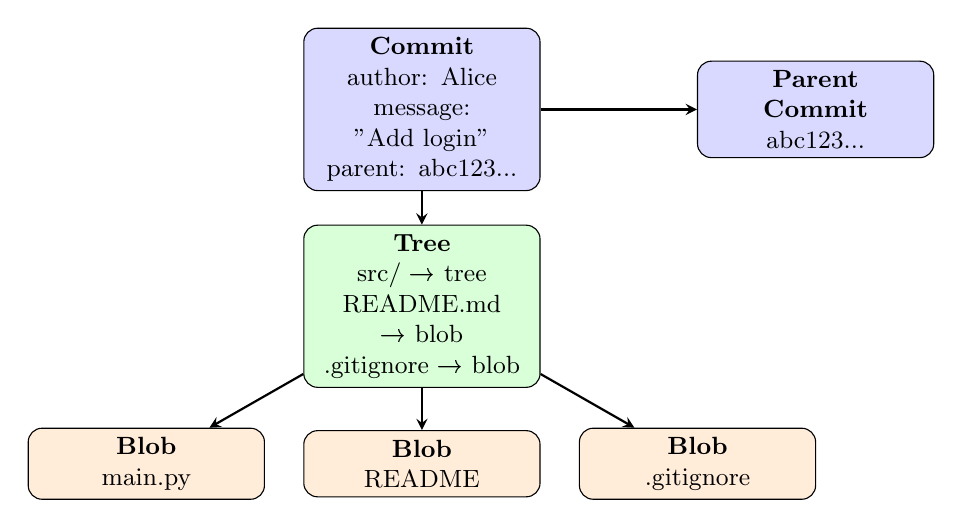
\begin{tikzpicture}[
  obj/.style={draw, rounded corners=5pt, minimum width=3cm, minimum height=0.8cm,
              font=\small, align=center, text width=2.5cm},
  hash/.style={font=\tiny\ttfamily, color=gray},
  arr/.style={->, thick, >=stealth}
]
  % Commit node
  \node[obj, fill=blue!15, minimum height=1.5cm] (commit) at (0,0) {
    \textbf{Commit}\\
    author: Alice\\
    message: "Add login"\\
    parent: abc123...
  };

  % Tree node
  \node[obj, fill=green!15] (tree) at (0,-2.5) {
    \textbf{Tree}\\
    src/ → tree\\
    README.md → blob\\
    .gitignore → blob
  };

  % Blob nodes
  \node[obj, fill=orange!15] (blob1) at (-3.5,-4.5) {\textbf{Blob}\\main.py};
  \node[obj, fill=orange!15] (blob2) at (0,-4.5) {\textbf{Blob}\\README};
  \node[obj, fill=orange!15] (blob3) at (3.5,-4.5) {\textbf{Blob}\\.gitignore};

  % Parent commit
  \node[obj, fill=blue!15, minimum height=1cm] (parent) at (5,0) {
    \textbf{Parent Commit}\\
    abc123...
  };

  \draw[arr] (commit) -- (tree);
  \draw[arr] (tree) -- (blob1);
  \draw[arr] (tree) -- (blob2);
  \draw[arr] (tree) -- (blob3);
  \draw[arr] (commit) -- (parent);
\end{tikzpicture}%
}
\caption{一次提交的完整数据模型——Commit 指向 Tree，Tree 指向 Blob，并记录父提交}\label{fig:commit-structure}\end{figure}

\begin{infobox}
\textbf{用底层命令查看对象}：

Git 提供了底层命令来直接查看四种对象的内容：
\begin{lstlisting}[style=shellinbox]
git cat-file -p HEAD          # 查看 HEAD 指向的 Commit 对象
git cat-file -p HEAD^{tree}   # 查看该 Commit 对应的 Tree 对象
git ls-tree HEAD              # 列出 Tree 中的文件与 Blob 映射
git cat-file -p <blob-hash>   # 查看 Blob 的内容
\end{lstlisting}
\end{infobox}

\begin{infobox}
\textbf{为什么 Git 高效？}
\begin{itemize}
  \item \textbf{快照式存储}：每次提交保存完整快照，未修改的文件复用旧 Blob（通过哈希判断）。
  \item \textbf{指针轻量}：分支只是一个 40 字节的指针，创建分支几乎不消耗空间。
  \item \textbf{本地完整}：每个克隆都包含完整历史，无需联网即可查看和操作。
  \item \textbf{自动垃圾回收}：Git 定期运行 \texttt{git gc}，将松散对象（loose objects）
        打包为 packfile 和索引文件，通过 delta 压缩进一步节省存储空间。
\end{itemize}
\end{infobox}

\begin{tipbox}
\textbf{Porcelain vs Plumbing}：

Git 命令分为两层\textbf{表层（Porcelain）}是你日常使用的命令（\texttt{git add}、
\texttt{git commit}、\texttt{git log}），设计为人类友好；\textbf{底层（Plumbing）}是 Git
内部使用的命令（\texttt{git cat-file}、\texttt{git hash-object}、\texttt{git ls-tree}），
输出格式稳定，适合脚本调用。理解数据模型时，底层命令是最好的"显微镜"。

日常工作中你几乎不需要直接使用 Plumbing 命令，但了解它们能帮你深入诊断问题。
\end{tipbox}

\section{GitHub 简介}

\textbf{GitHub} 是全球最大的代码托管平台（2018 年被微软收购），截至 2025 年已有超过 1 亿开发者用户。
它为 Git 仓库提供云端托管服务。Git 与 GitHub 的对比如表~\ref{tab:git-vs-github} 所示：

\begin{infobox}[boxsep=2mm, left=6mm, right=6mm]
\captionof{table}{Git vs GitHub 的区别}\label{tab:git-vs-github}

{\renewcommand{\arraystretch}{1.3}\setlength{\tabcolsep}{6pt}\begin{tabularx}{\linewidth}{l >{\raggedright\arraybackslash}X >{\raggedright\arraybackslash}X}
\toprule
& \textbf{Git} & \textbf{GitHub} \\
\midrule
本质 & 命令行工具（软件） & 云端服务（网站） \\
类比 & 像"发邮件"这个动作 & 像"Gmail"这个服务 \\
运行位置 & 你的电脑上 & github.com 服务器上 \\
是否需要联网 & 不需要 & 需要 \\
替代品 & Mercurial, SVN & GitLab, Bitbucket, Gitee \\
\bottomrule
\end{tabularx}}
\end{infobox}

GitHub 提供的核心功能包括：

\begin{itemize}[leftmargin=2em]
  \item \textbf{远程仓库托管}（云端备份库）：将本地 Git 仓库同步到云端，实现备份和多设备协作。
  \item \textbf{Pull Request}（PR，合并申请：请求把分支合并到主分支）：代码审查与合并请求机制，是团队协作的核心流程。
  \item \textbf{Issue 管理}：内建的任务追踪和 Bug 报告系统。
  \item \textbf{GitHub Actions}：CI/CD 自动化流水线，支持自动测试和部署。
  \item \textbf{Pages}：免费的静态网站托管服务。
  \item \textbf{Copilot}：AI 辅助编程工具，集成在编辑器中。
\end{itemize}

\section{Git 的三大工作区域}

理解 Git 的关键在于理解它的\textbf{三个工作区域}。所有 Git 操作本质上都是在这三个区域之间移动数据。
这是学习 Git 最重要的一张图，请务必理解，如图~\ref{fig:three-zones} 所示：

\begin{figure}[H]\centering
\resizebox{\textwidth}{!}{%
\begin{tikzpicture}[
  box/.style={draw, rounded corners=8pt, minimum width=3.5cm, minimum height=1.5cm,
              font=\bfseries, align=center, text width=3cm, fill=#1},
  arr/.style={->, thick, >=stealth},
  node distance=1.2cm
]
  \node[box=red!15] (work) {工作区\\(Working Directory)\\{\small 磁盘上的文件}};
  \node[box=yellow!15, right=1cm of work] (stage) {暂存区\\(Staging Area / Index)\\{\small 准备提交的变更}};
  \node[box=green!15, right=1cm of stage] (repo) {本地仓库\\(Repository)\\{\small 已提交的历史}};
  \node[box=blue!15, right=1cm of repo] (remote) {远程仓库\\(Remote)\\{\small GitHub 上的副本}};

  \draw[arr] (work) -- node[above, font=\small, align=center]{git add\\{\tiny 暂存变更}} (stage);
  \draw[arr] (stage) -- node[above, font=\small, align=center]{git commit\\{\tiny 提交快照}} (repo);
  \draw[arr] (repo) -- node[above, font=\small, align=center]{git push\\{\tiny 推送到远程}} (remote);
  \draw[arr] (remote) -- node[below, font=\small, align=center]{git pull / fetch\\{\tiny 拉取更新}} (work);
\end{tikzpicture}
}
\caption{Git 三大工作区域与远程仓库——工作区、暂存区、本地仓库、远程仓库之间的数据流转}\label{fig:three-zones}\end{figure}

\begin{itemize}[leftmargin=2em]
  \item \textbf{工作区}（Working Directory）：你在磁盘上看到的实际文件，可以直接编辑。
        就是你在 VS Code 中打开的那些文件。
  \item \textbf{暂存区}（购物车：选好要结账的商品；Staging Area / Index）：一个准备提交的变更列表。通过 \texttt{git add}
        将文件放入暂存区，只有暂存区的内容才会被包含在下一次提交中。
        \textbf{暂存区是 Git 独有的设计}——它让你可以精确选择"这次提交包含哪些修改"。
  \item \textbf{本地仓库}（Repository）：Git 的 \texttt{.git} 目录，存储了所有提交的完整历史。
        这是 Git 的"大脑"，删除它等于删除所有版本历史。
  \item \textbf{远程仓库}（Remote）：托管在 GitHub 等服务器上的仓库副本。
        用于团队间的代码共享和备份。
\end{itemize}

\begin{tipbox}
\textbf{类比理解}：把 Git 想象成拍照。
\begin{itemize}
  \item \textbf{工作区} = 你眼前的场景（随时在变）
  \item \textbf{暂存区} = 取景框（你选择要拍什么）
  \item \textbf{提交} = 按下快门（保存一个不可变的快照）
\end{itemize}
\end{tipbox}

\section{VS Code 如何与 Git 协作}

VS Code 内置了强大的 Git 集成，将上述所有操作都图形化了。如图~\ref{fig:sc-overview} 所示，VS Code 源代码管理视图
的全貌——你将在本教程中反复看到这个界面：

\vscodeimg{images/01-sc-overview.png}{VS Code 源代码管理视图全景——左侧为变更文件列表，上方为提交信息输入框和提交按钮。这是你与 Git 交互的主要界面}{fig:sc-overview}

在 VS Code 中，你可以通过\textbf{点击按钮}完成大部分 Git 操作，而不必记住命令行语法。
但理解底层命令仍然重要——它们帮助你诊断问题、执行高级操作。

\begin{tipbox}
\textbf{本章小结}
\begin{itemize}
  \item 版本控制系统记录文件变更历史，支持协作、回退和并行开发
  \item Git 是分布式版本控制系统，每个克隆都包含完整历史
  \item Git 使用 Blob、Tree、Commit、Branch 四种对象存储数据
  \item GitHub 是云端托管平台，为 Git 仓库提供远程存储和协作功能
  \item Git 的三大工作区域：工作区 → 暂存区 → 本地仓库 → 远程仓库
  \item VS Code 内置了强大的 Git 集成，将命令行操作图形化
\end{itemize}

\textbf{下一章预告}：我们将学习如何安装 Git 和 VS Code，以及如何配置 GitHub 认证。
\end{tipbox}

\subsection*{动手实验 1：初始化第一个仓库}

花 5 分钟亲手创建本章反复提到的「仓库」。本实验全程只使用鼠标点击，不需要输入任何命令。

\medskip
\begin{enumerate}[leftmargin=1.5em]
  \item 在桌面空白处单击鼠标右键，选择「新建」$\to$「文件夹」，输入名称 \texttt{my-first-repo} 并回车。
  \item 打开 VS Code，点击菜单栏「文件」$\to$「打开文件夹…」，选中 \texttt{my-first-repo} 文件夹，点击「选择文件夹」按钮。
  \item 按 \texttt{Ctrl+Shift+G} 打开源代码管理视图，点击「初始化仓库」按钮。
  \item 在左侧资源管理器点击「新建文件」图标，输入文件名 \texttt{hello.txt} 并回车；在编辑器中输入文字 \texttt{Hello Git!}，按 \texttt{Ctrl+S} 保存。
  \item 回到源代码管理视图，观察 \texttt{hello.txt} 出现在「更改」列表中并带有 \texttt{U} 标记（Untracked，未跟踪），说明仓库已初始化成功。
\end{enumerate}
\medskip

\begin{tipbox}
\textbf{成功标志}：打开 Windows 资源管理器进入 \texttt{my-first-repo} 文件夹，点击菜单栏「查看」$\to$ 勾选「隐藏的项目」，可以看到 \texttt{.git} 文件夹。
这个仓库会一直用于第 3、4 章的动手实验。
\end{tipbox}

% ================================================================
%  第二章：Git 安装与配置
% ================================================================
\chapter{Git 安装与配置}

\begin{infobox}
\textbf{本章学习目标}
\begin{enumerate}[leftmargin=1.5em]
  \item 在不同操作系统上安装 Git
  \item 配置 Git 的用户信息和偏好设置
  \item 安装和配置 VS Code
  \item 配置 GitHub 认证（SSH 和 Token）
\end{enumerate}
\end{infobox}

\section{安装 Git}

\begin{infobox}
\textbf{Git 版本选择建议}

Git 是一个持续更新的工具，新版本通常修复了旧版本的 bug 并增加了功能。
\begin{itemize}
  \item \textbf{Windows}：建议从官网下载最新版（通常每几个月更新一次）
  \item \textbf{macOS}：通过 Homebrew 安装可以方便地更新（\texttt{brew upgrade git}）
  \item \textbf{Linux}：系统包管理器中的版本可能较旧，如需最新版可从官网下载源码编译
\end{itemize}

本书基于 Git 2.40+ 版本编写，但绝大多数操作在所有现代 Git 版本中都相同。
\end{infobox}

\subsection{Windows 系统}

\medskip
\begin{enumerate}[leftmargin=1.5em]
  \item 访问 Git 官网 \url{https://git-scm.com/download/win}，下载 Windows 安装包。
  \item 运行安装程序，大部分选项保持默认即可。\textbf{建议注意以下选项}：
  \begin{itemize}
    \item \textbf{默认编辑器}：选择"Use Visual Studio Code as Git's default editor"。
    \item \textbf{PATH 环境}：选择"Git from the command line and also from 3rd-party software"，
          这样可以在 PowerShell、CMD 等任何终端中使用 Git。
    \item \textbf{HTTPS 传输后端}：选择"Use the OpenSSL library"。
    \item \textbf{行尾符号}：选择"Checkout Windows-style, commit Unix-style line endings"。
          这能避免 Windows 和 Linux/macOS 之间的换行符冲突。
  \end{itemize}
  \item 安装完成后，打开 PowerShell，验证安装：
\end{enumerate}
\medskip

\begin{lstlisting}[style=shell]
# 验证 Git 安装
git --version
# 输出示例：git version 2.45.0.windows.1
\end{lstlisting}

\subsection{macOS 系统}

\begin{lstlisting}[style=shell]
# 方法一：通过 Xcode Command Line Tools（首次运行 git 时自动提示）
xcode-select --install

# 方法二：通过 Homebrew（推荐，版本更新）
brew install git
\end{lstlisting}

\subsection{Linux 系统}

\begin{lstlisting}[style=shell]
# Debian / Ubuntu
sudo apt update && sudo apt install git

# Fedora / RHEL
sudo dnf install git

# Arch Linux
sudo pacman -S git
\end{lstlisting}

\section{基本配置}

安装 Git 后，第一件事是配置你的身份信息和偏好设置。这些配置会附加在你每次提交上，
相当于给每次修改"签名"。

\begin{infobox}
\textbf{为什么需要配置用户信息？}

Git 是分布式版本控制系统，每次提交都会记录"谁"做了这次修改。如果没有配置用户信息，
Git 会拒绝提交，并提示你设置 \texttt{user.name} 和 \texttt{user.email}。

这些信息会被永久记录在提交历史中，用于：
\begin{itemize}
  \item 追溯代码的作者（\texttt{git log} 和 \texttt{git blame}）
  \item 与 GitHub/GitLab 等平台的账号关联
  \item 生成贡献统计图表
\end{itemize}
\end{infobox}

\subsection{用户身份（必须配置）}

\begin{lstlisting}[style=shell]
# 设置全局用户名（显示在提交记录中）
git config --global user.name "你的名字"

# 设置全局邮箱（必须与 GitHub 账号邮箱一致）
git config --global user.email "your.email@example.com"
\end{lstlisting}

\begin{keybox}
\textbf{配置原理}：这些设置被存储在你的用户目录下的 \texttt{.gitconfig} 文件中（Windows 在 
\texttt{C:\\Users\\你的用户名\\.gitconfig}，macOS/Linux 在 \texttt{\textasciitilde/.gitconfig}）。

每次执行 \texttt{git commit} 时，Git 会读取这个文件，将用户名和邮箱写入提交记录中。
你可以随时用 \texttt{git config --global --list} 查看当前配置。
\end{keybox}

\begin{warnbox}
邮箱地址必须与你的 GitHub 账号关联的邮箱一致，否则 GitHub 无法将提交与你的账号关联。
可以在 GitHub 的 Settings $\to$ Emails 中查看你的邮箱。
\end{warnbox}

\subsection{其他推荐配置}

以下配置能显著提升日常使用体验：

\begin{lstlisting}[style=shell]
# 设置默认分支名为 main（GitHub 的默认分支名）
git config --global init.defaultBranch main

# 设置默认编辑器为 VS Code（这样 git commit 会打开 VS Code 写提交信息）
git config --global core.editor "code --wait"

# 设置 pull 时使用 rebase（保持线性历史，推荐）
git config --global pull.rebase true

# 设置常用别名，简化命令输入
git config --global alias.st status          # git st = git status
git config --global alias.co checkout        # git co = git checkout
git config --global alias.br branch          # git br = git branch
git config --global alias.ci commit          # git ci = git commit
git config --global alias.lg "log --oneline --graph --all"
                                              # git lg = 图形化日志

# 查看当前所有配置
git config --list
\end{lstlisting}

\subsection{配置层级}

Git 配置有三个层级，优先级从高到低：（见表~\ref{tab:config-levels}）

\begin{table}[h]
\centering
\caption{Git 配置的三个层级}\label{tab:config-levels}
\begin{tabularx}{\textwidth}{l l >{\raggedright\arraybackslash}X}
\toprule
\textbf{层级} & \textbf{存储位置} & \textbf{作用范围} \\
\midrule
\texttt{--local} & 仓库的 \texttt{.git/config} & 仅当前仓库生效 \\
\texttt{--global} & \texttt{\~{}/.gitconfig} & 当前用户所有仓库生效 \\
\texttt{--system} & \texttt{/etc/gitconfig} & 系统所有用户生效 \\
\bottomrule
\end{tabularx}
\end{table}

\begin{tipbox}
日常使用中，绝大多数配置使用 \texttt{--global} 即可。如果某个项目需要特殊配置
（比如用公司邮箱提交），在该仓库目录下不加 \texttt{--global} 即可覆盖全局设置。
例如：\texttt{git config user.email "work@company.com"}（仅影响当前仓库）。
\end{tipbox}

\section{安装 VS Code}

VS Code（Visual Studio Code）是微软开发的免费代码编辑器，内置了强大的 Git 集成。

\begin{infobox}
\textbf{为什么选择 VS Code？}

VS Code 之所以成为最受欢迎的代码编辑器之一，除了免费开源外，还有以下优势：
\begin{itemize}
  \item \textbf{内置 Git 集成}：无需额外安装插件，开箱即用
  \item \textbf{直观的 Diff 视图}：清晰展示文件修改前后的对比
  \item \textbf{图形化冲突解决}：用颜色标记冲突区域，一键选择保留哪边
  \item \textbf{丰富的扩展生态}：GitLens、Git Graph 等扩展进一步增强了 Git 体验
  \item \textbf{跨平台}：Windows、macOS、Linux 都有完全一致的界面和操作
\end{itemize}
\end{infobox}

\medskip
\begin{enumerate}[leftmargin=1.5em]
  \item 访问 \url{https://code.visualstudio.com/} 下载并安装。
  \item 安装时勾选"将 Code 注册为受支持的文件类型的编辑器"和"添加到 PATH"。
  \item 安装完成后，可以通过命令行 \texttt{code .} 在当前目录打开 VS Code。
\end{enumerate}
\medskip

\section{配置 GitHub 认证}

VS Code 与 GitHub 集成需要认证。推荐使用以下方式之一：

\subsection{方式一：GitHub CLI（推荐）}

\begin{lstlisting}[style=shell]
# 安装 GitHub CLI（https://cli.github.com/）
# Windows: winget install GitHub.cli
# macOS: brew install gh

# 登录 GitHub
gh auth login
# 按提示选择：GitHub.com -> HTTPS -> Login with browser
\end{lstlisting}

\subsection{方式二：Personal Access Token}

\medskip
\begin{enumerate}[leftmargin=1.5em]
  \item 登录 GitHub $\to$ Settings $\to$ Developer settings $\to$
        Personal access tokens $\to$ Tokens (classic)。
  \item 点击"Generate new token (classic)"，勾选 \texttt{repo} 权限。
  \item 复制生成的 token，在 Git 提示输入密码时粘贴。
  \item 建议使用 \texttt{git credential-manager} 保存凭据，避免重复输入。
\end{enumerate}
\medskip

\begin{tipbox}
VS Code 首次连接 GitHub 时，会自动弹出登录提示，引导你通过浏览器完成 OAuth 认证。
认证成功后，VS Code 会自动管理 token，无需手动配置。
\end{tipbox}

\subsection{方式三：SSH 密钥（最推荐）}

SSH 密钥认证是最安全、最方便的 GitHub 认证方式。配置一次后，无需每次都输入密码。

\textbf{配置 SSH 密钥}：
\medskip
\begin{enumerate}[leftmargin=1.5em]
  \item 打开终端，生成 SSH 密钥（使用你的 GitHub 邮箱）：
\begin{lstlisting}[style=shellinbox]
# 生成 SSH 密钥（使用你的 GitHub 邮箱）
ssh-keygen -t ed25519 -C "your.email@example.com"

# 按 Enter 接受默认保存位置
# 输入并确认一个密码（可选，但推荐）
\end{lstlisting}
  \item 将 SSH 密钥添加到 ssh-agent：
\begin{lstlisting}[style=shellinbox]
# 启动 ssh-agent
eval "$(ssh-agent -s)"

# 添加私钥到 ssh-agent
ssh-add ~/.ssh/id_ed25519
\end{lstlisting}
  \item 复制公钥内容：
\begin{lstlisting}[style=shellinbox]
# 复制公钥到剪贴板（macOS）
pbcopy < ~/.ssh/id_ed25519.pub

# 或手动复制（Windows / Linux）
cat ~/.ssh/id_ed25519.pub
# 然后手动复制输出内容
\end{lstlisting}
  \item 在 GitHub 网页上添加公钥：
  \begin{itemize}
    \item 登录 GitHub $\to$ Settings $\to$ SSH and GPG keys
    \item 点击 "New SSH key"
    \item 粘贴公钥内容，给密钥起个描述性标题（如 "My Laptop"）
    \item 点击 "Add SSH key"
  \end{itemize}
  \item 测试连接：
\begin{lstlisting}[style=shellinbox]
ssh -T git@github.com
# 看到 "Hi username! You've successfully authenticated..." 表示成功
\end{lstlisting}
\end{enumerate}
\medskip

\begin{keybox}
\textbf{HTTPS vs SSH 对比}：
\begin{itemize}
  \item \textbf{HTTPS}：使用用户名+密码（或 Token）认证。适合临时使用，但频繁推送时需要输入凭据。
  \item \textbf{SSH}：使用密钥对认证。配置一次后免密操作，适合长期开发。
\end{itemize}
\textbf{推荐}：个人开发使用 SSH，团队协作可配合使用 HTTPS。
\end{keybox}

\subsection*{动手实验 2：配置用户身份和SSH密钥}

花 5 分钟完成身份配置并添加 SSH 密钥。本实验全程只使用鼠标和浏览器，不需要输入命令。
配置后你的每次提交都会正确显示作者身份，并且可以用 SSH 免密访问 GitHub。

\medskip
\begin{enumerate}[leftmargin=1.5em]
  \item 打开 VS Code，按 \texttt{Ctrl+O}（打开文件），在输入框粘贴路径 \texttt{C:\textbackslash Users\textbackslash 你的用户名\textbackslash .gitconfig}，点击「打开」；若提示文件不存在，点击弹窗中的「创建文件」按钮。
  \item 在文件中输入以下内容（把名字和邮箱换成你自己的，邮箱须与 GitHub 账号一致），按 \texttt{Ctrl+S} 保存：
\begin{lstlisting}[style=shell]
[user]
	name = 你的名字
	email = your.email@example.com
\end{lstlisting}
  \item 打开浏览器登录 \url{https://github.com}，点击右上角头像 $\to$「Settings」$\to$ 左侧菜单「SSH and GPG keys」。
  \item 点击绿色按钮「New SSH key」，在 Title 输入框输入 \texttt{My Laptop}。
  \item 在 Key 输入框粘贴第 2 章生成的公钥内容（\texttt{id\_ed25519.pub} 文件的内容），点击「Add SSH key」完成添加。
\end{enumerate}
\medskip

\begin{tipbox}
\textbf{成功标志}：SSH 密钥页面出现名为 \texttt{My Laptop} 的密钥记录；
同时 VS Code 中提交信息会显示你在 \texttt{.gitconfig} 中填写的名字和邮箱。
\end{tipbox}

% ================================================================
%  第三章：Git 基础操作
% ================================================================
\chapter{Git 基础操作}

\begin{infobox}
\textbf{本章学习目标}
\begin{enumerate}[leftmargin=1.5em]
  \item 掌握仓库的初始化和克隆操作
  \item 理解文件的四种状态及其转换关系
  \item 熟练使用 status、add、commit 等核心命令
  \item 掌握 diff 视图的三种对比模式
  \item 学会撤销和回退操作
  \item 配置 .gitignore 文件
\end{enumerate}
\end{infobox}

本章介绍 Git 最核心的日常操作。无论你使用命令行还是 VS Code 图形界面，
底层执行的都是这些命令。理解它们，你就能在任何场景下灵活应对。

\section{初始化仓库}

每个 Git 项目都始于一个\textbf{仓库}（Repository）。

\begin{infobox}
\textbf{什么是仓库？}

你可以把"仓库"理解为一个"时间胶囊"——它不仅存储了你当前的文件，还存储了这些文件的每一次修改记录。当你对一个文件进行修改、保存、提交后，Git 会把这次修改记录下来，就像一个时间戳，标记着"在这个时刻，文件是这样的"。

初始化仓库，就是告诉 Git："从现在开始，请帮我记录这个文件夹里所有文件的变化历史。"
\end{infobox}

有两种方式创建仓库：

\subsection{方式一：在已有项目中初始化}

如果你已经有一个项目文件夹，想将它纳入 Git 管理：

\begin{lstlisting}[style=shell]
# 进入项目目录
cd my-project

# 初始化 Git 仓库（创建 .git 目录）
git init

# 此时目录中会出现一个隐藏的 .git 文件夹
# 这就是 Git 存储所有历史数据的地方
\end{lstlisting}

在 VS Code 中，操作更加直观——打开项目文件夹后，源代码管理视图会自动检测到
这不是一个 Git 仓库，并显示"初始化仓库"按钮，如图~\ref{fig:init-repo} 所示：

\vscodeimg{images/12-init-repo.png}{VS Code 中的"初始化仓库"按钮——打开一个非 Git 项目时，源代码管理视图会提示你初始化}{fig:init-repo}

点击后，VS Code 会在项目根目录执行 \texttt{git init}，创建 \texttt{.git} 目录。
此时你会看到所有项目文件出现在"更改"列表中，状态为 \texttt{U}（Untracked，未跟踪）。

\subsection{方式二：克隆远程仓库}

如果项目已经存在于 GitHub 等远程平台，使用 \texttt{git clone}（克隆：把云端仓库完整下载到本地）将完整仓库下载到本地：

\begin{lstlisting}[style=shell]
# 克隆远程仓库到本地
git clone https://github.com/username/repo-name.git

# 克隆到指定目录
git clone https://github.com/username/repo-name.git my-folder

# 克隆时指定分支
git clone -b develop https://github.com/username/repo-name.git
\end{lstlisting}

在 VS Code 中，可以通过命令面板执行克隆操作，如图~\ref{fig:clone-repo} 所示：

\vscodeimg{images/11-clone-repo.png}{VS Code 的 Git: Clone 命令——按 Ctrl+Shift+P 输入"clone"，粘贴仓库 URL 即可克隆}{fig:clone-repo}

\begin{infobox}
\texttt{git clone} 实际上做了三件事：
\begin{enumerate}
  \item 从远程下载完整的仓库历史到本地（包括所有分支和提交）
  \item 创建名为 \texttt{origin} 的远程引用指向原仓库
  \item 自动检出（checkout）默认分支（通常是 \texttt{main}）的文件到工作区
\end{enumerate}
\end{infobox}

\section{文件状态与跟踪}

Git 中的文件有四种状态，理解这些状态是掌握 Git 的基础：如表~\ref{tab:file-states} 所示。

\begin{table}[h]
\centering
\caption{Git 中文件的四种状态}\label{tab:file-states}
\begin{tabularx}{\textwidth}{l l >{\raggedright\arraybackslash}X}
\toprule
\textbf{状态} & \textbf{标记} & \textbf{含义} \\
\midrule
Untracked（未跟踪） & \texttt{??} & 新文件，Git 尚未纳入管理，不会出现在提交中 \\
Unmodified（未修改） & 无标记 & 已跟踪，且自上次提交后未修改 \\
Modified（已修改） & \texttt{M} & 已跟踪，但内容已被修改，需要决定是否提交 \\
Staged（已暂存） & \texttt{A} / \texttt{M} & 修改已放入暂存区，将在下次提交时保存 \\
\bottomrule
\end{tabularx}
\end{table}

文件状态的生命周期如图~\ref{fig:file-states} 所示：

\begin{figure}[H]\centering
\resizebox{\textwidth}{!}{%
\begin{tikzpicture}[
  state/.style={draw, rounded corners=8pt, minimum width=3.5cm, minimum height=1.2cm,
                font=\small, align=center, text width=3cm, fill=#1},
  arr/.style={->, thick, >=stealth},
  node distance=1.5cm
]
  % States
  \node[state=gray!15] (untracked) at (0,0) {未跟踪\\(Untracked)};
  \node[state=yellow!20] (modified) at (4,0) {已修改\\(Modified)};
  \node[state=green!20] (staged) at (8,0) {已暂存\\(Staged)};
  \node[state=blue!20] (unmodified) at (4,-2.5) {未修改\\(Unmodified)};

  % Arrows
  \draw[arr] (untracked) -- node[above, font=\small]{git add} (staged);
  \draw[arr] (modified) -- node[above, font=\small]{git add} (staged);
  \draw[arr] (staged) -- node[right, font=\small]{git commit} (unmodified);
  \draw[arr, dashed] (unmodified) -- node[left, font=\small]{编辑文件} (modified);
  \draw[arr] (unmodified) -- ++(4,0) -- ++(0,2.5) -- node[right, font=\small]{删除文件} (untracked);

  % Legend
  \node[anchor=west, font=\small, text width=14cm, align=center] at (0,-3.5) {
    \textbf{说明}：新建文件 → git add → 已暂存 → git commit → 未修改 → 编辑 → 已修改 → git add → ...
  };
\end{tikzpicture}
}
\caption{文件状态生命周期——未跟踪、已修改、已暂存、未修改之间的转换关系}\label{fig:file-states}\end{figure}

\section{日常工作流：status → add → commit}

这是你最频繁使用的 Git 操作循环——\textbf{修改文件 → 暂存 → 提交}，每天会重复几十次。

\subsection{第一步：查看状态（git status）}

\begin{lstlisting}[style=shell]
# 查看仓库状态（最常用！）
git status

# 简洁输出（推荐日常使用）
git status -s

# 示例输出：
#  M modified-file.txt    ← 已修改，未暂存（红色）
# A  new-file.txt         ← 新文件，已暂存（绿色）
# ?? untracked.txt        ← 未跟踪的文件（红色）
\end{lstlisting}

在 VS Code 中，\texttt{git status} 的信息直接体现在源代码管理视图里，如图~\ref{fig:modified-files} 所示：

\vscodeimg{images/13-modified-files.png}{修改后的文件列表——源代码管理视图的"更改"区域显示所有已修改但未暂存的文件，每个文件旁有状态标记}{fig:modified-files}

图~\ref{fig:modified-files} 中，你可以看到：
\begin{itemize}[leftmargin=2em]
  \item 每个修改过的文件都列在"更改"区域下
  \item 文件名右侧的字母表示状态（M = Modified，U = Untracked）
  \item 点击文件名可以打开差异对比视图，查看具体改了什么
\end{itemize}

\begin{tipbox}
\texttt{git status} 是你最应该频繁执行的命令。它告诉你当前处于什么状态，
哪些文件需要处理。养成"做任何操作前先 status"的习惯。
在 VS Code 中，状态信息始终可见——源代码管理视图就是实时的 \texttt{git status}。
\end{tipbox}

\subsection{第二步：暂存文件（git add）}

暂存是 Git 独有的设计——它让你在提交之前\textbf{精确选择}要包含哪些修改。

\begin{lstlisting}[style=shell]
# 暂存单个文件
git add filename.txt

# 暂存多个文件
git add file1.txt file2.txt file3.txt

# 暂存当前目录下所有变更（包括新文件和修改）
git add .

# 暂存指定目录
git add src/

# 查看暂存区中具体有哪些变更
git diff --cached
\end{lstlisting}

在 VS Code 中，暂存操作就是点击文件旁边的 "+" 按钮（单个暂存），或点击"更改"标题右侧的 "+" 按钮（全部暂存），如图~\ref{fig:stage-changes} 所示：

\vscodeimg{images/05-stage-changes.png}{暂存操作——点击文件右侧的 "+" 按钮暂存单个文件，或点击"更改"标题旁的"+"按钮全部暂存}{fig:stage-changes}

\begin{warnbox}
\texttt{git add .}（或 VS Code 中的全部暂存按钮）会暂存\textbf{所有}变更，
包括你可能不想提交的文件（如临时文件、密钥文件等）。
请务必先用 \texttt{git status} 确认，并通过 \texttt{.gitignore} 文件排除不需要的文件。
\end{warnbox}

\subsection{第三步：提交变更（git commit）}

\begin{lstlisting}[style=shell]
# 提交暂存区的变更（会打开编辑器让你写提交信息）
git commit

# 直接在命令行写提交信息
git commit -m "添加用户登录功能"

# 提交所有已跟踪文件的修改（跳过 git add 步骤）
git commit -a -m "修复样式问题"
\end{lstlisting}

在 VS Code 中，提交操作分两步：输入提交信息 → 点击提交按钮，如图~\ref{fig:commit-button} 所示。

\vscodeimg{images/15-commit-button.png}{提交操作——在顶部输入框填写提交信息，然后点击"提交"按钮（或按 Ctrl+Enter）完成提交}{fig:commit-button}

提交后，"暂存的更改"区域清空，变更进入本地历史记录。

\subsection{编写好的提交信息}

提交信息（commit message）是 Git 历史中最重要的文档。好的提交信息应该：

\begin{itemize}[leftmargin=2em]
  \item \textbf{第一行}：简明扼要地描述变更（不超过 50 个字符），使用祈使语气。
  \item \textbf{空一行}后（可选）：详细描述\textbf{为什么}做这个改动，而不仅仅是做了什么。
\end{itemize}

\begin{lstlisting}[style=shell]
# 好的提交信息示例
git commit -m "修复购物车总价计算精度问题"
git commit -m "添加用户头像上传功能"
git commit -m "重构数据库连接池配置"

# 差的提交信息示例
git commit -m "fix"              # 太模糊——修了什么？
git commit -m "update"           # 更新了什么？
git commit -m "asdfasdf"         # 无意义
git commit -m "修复了bug，改了三个文件，还加了一个功能"  # 太杂，应拆分为多个提交
\end{lstlisting}

\begin{tipbox}
VS Code 支持 AI 辅助生成提交信息——点击提交信息输入框旁的"魔法棒"图标，
VS Code 会根据你的代码变更自动生成描述。你可以在此基础上修改，也可以直接采纳。
\end{tipbox}

\section{查看修改内容：Diff 视图}

在提交之前，你应该先检查自己到底改了什么。VS Code 提供了强大的可视化差异对比功能。

\subsection{打开 Diff 视图}

在源代码管理视图中，\textbf{点击文件名}即可打开差异对比视图，如图~\ref{fig:diff-editor} 所示：

\vscodeimg{images/03-diff-editor.png}{差异对比编辑器——左侧为旧版本（HEAD），右侧为当前修改。绿色背景表示新增内容，红色背景表示删除内容}{fig:diff-editor}

\subsection{并排视图 vs 内联视图}

VS Code 支持两种差异对比模式，点击 Diff 编辑器右上角的按钮可以切换：

\begin{itemize}[leftmargin=2em]
  \item \textbf{并排视图（Side-by-Side）}：左右分栏显示两个版本，适合大幅修改。
  \item \textbf{内联视图（Inline）}：所有变更在同一文件中显示，适合小改动。
\end{itemize}

两种模式的对比如图~\ref{fig:diff-sidebyside} 与图~\ref{fig:diff-inline} 所示——并排视图可以一目了然地看到左右差异，而内联视图则更紧凑：

\vspace{0.5cm}
\noindent
\begin{minipage}[t]{0.48\textwidth}
\vscodeimgnarrow{images/24-diff-sidebyside.png}{并排视图——左右分栏，适合大幅修改}{fig:diff-sidebyside}
\end{minipage}
\hfill
\begin{minipage}[t]{0.48\textwidth}
\vscodeimgnarrow{images/25-diff-inline.png}{内联视图——变更在同一文件中显示，适合小改动}{fig:diff-inline}
\end{minipage}
\vspace{0.5cm}

\subsection{编辑器中的实时变更指示}

在代码编辑器中，VS Code 会在行号右侧的 gutter 区域\textbf{实时}显示变更指示，如图~\ref{fig:gutter-diff} 所示：

\vscodeimg{images/21-gutter-diff.png}{编辑器 Gutter 变更指示器——绿色竖线表示新增行，蓝色竖线表示修改行，红色三角表示删除行。点击可查看详细信息}{fig:gutter-diff}

\begin{itemize}[leftmargin=2em]
  \item \textbf{绿色竖线}：新增的行
  \item \textbf{蓝色竖线}：修改的行
  \item \textbf{红色三角}：删除的行（行号旁的小三角）
\end{itemize}

\textbf{点击这些指示器}，会弹出一个小浮窗，显示该行的详细变更内容，并提供"撤销此更改"的快捷操作。

\subsection{命令行 diff 详解}

除了 VS Code 的可视化 diff，命令行的 \texttt{git diff} 也非常强大。掌握以下常用用法：

\begin{lstlisting}[style=shell]
# 查看工作区与暂存区的差异（未暂存的修改）
git diff

# 查看暂存区与最后一次提交的差异（已暂存的修改）
git diff --cached
git diff --staged  # 同上

# 查看工作区与最后一次提交的所有差异（暂存+未暂存）
git diff HEAD

# 查看两次提交之间的差异
git diff abc123..def456

# 查看某个文件的差异
git diff filename.txt

# 查看某次提交的完整变更
git diff abc123^..abc123
\end{lstlisting}

\begin{infobox}
\textbf{diff 的输出格式解读}：
\begin{lstlisting}[style=shellinbox]
--- a/filename.txt      # 旧版本（减号开头）
+++ b/filename.txt      # 新版本（加号开头）
@@ -1,5 +1,7 @@         # 变更位置：从第1行开始，旧版本5行，新版本7行
  unchanged line        # 无符号 = 未变更
-removed line           # 减号 = 删除的内容
+added line             # 加号 = 新增的内容
  unchanged line        # 上下文行，帮助定位
\end{lstlisting}
\end{infobox}

\section{查看历史：git log}

\begin{lstlisting}[style=shell]
# 基本日志（显示完整信息：作者、日期、提交信息）
git log

# 简洁模式：每行一个提交（推荐）
git log --oneline
# 输出示例：
# a1b2c3d 添加用户登录功能
# e4f5g6h 修复购物车计算bug
# i7j8k9l 初始化项目

# 图形化显示分支历史
git log --oneline --graph --all

# 查看最近 N 条提交
git log -5
git log --oneline -10

# 查看某个文件的修改历史
git log -p filename.txt

# 搜索提交信息
git log --grep="关键词"

# 查看某人的提交
git log --author="名字"

# 按时间范围
git log --since="2024-01-01" --until="2024-06-30"
\end{lstlisting}

\section{撤销操作}

Git 提供了多种撤销手段，适用于不同场景。这是初学者最容易困惑的部分，
但理解了"三个工作区域"的概念后，撤销操作就很好理解了。

\subsection{撤销工作区的修改（未 add）}

场景：你改了一个文件，但改错了，想恢复到上次提交的状态。

\begin{lstlisting}[style=shell]
# 丢弃工作区中对某个文件的修改（恢复到上次提交的状态）
git checkout -- filename.txt

# 或者使用更直观的新语法（Git 2.23+）
git restore filename.txt
\end{lstlisting}

\begin{warnbox}
这个操作是\textbf{不可逆}的！被撤销的修改无法恢复。请确认你真的不需要这些修改。
\end{warnbox}

\subsection{取消暂存（已 add，未 commit）}

场景：你暂存了文件，但发现暂存了不该暂存的文件，想把它从暂存区移回去。

\begin{lstlisting}[style=shell]
# 将文件从暂存区移回工作区（保留修改，只是不再暂存）
git reset HEAD filename.txt

# 或者使用新语法
git restore --staged filename.txt
\end{lstlisting}

\begin{tipbox}
在 VS Code 中，取消暂存就是点击"暂存的更改"区域中文件旁边的 "-" 按钮。
\end{tipbox}

\subsection{修改上一次提交}

场景：你刚提交完，发现提交信息写错了，或者忘了暂存某个文件。

\begin{lstlisting}[style=shell]
# 修改上一次提交的信息
git commit --amend -m "新的提交信息"

# 将新的修改追加到上一次提交中（不增加新提交）
git add forgotten-file.txt
git commit --amend --no-edit
\end{lstlisting}

\begin{warnbox}
\texttt{git commit --amend} 会改变提交的哈希值。如果这个提交已经推送到远程，
需要强制推送（\texttt{git push --force-with-lease}），谨慎使用。
\end{warnbox}

\subsection{回退到之前的版本}

\begin{lstlisting}[style=shell]
# 回退提交，保留修改在工作区（安全，推荐）
git reset --soft HEAD~1    # 回退1个提交，修改回到暂存区

# 回退提交，保留修改在工作区（未暂存）
git reset --mixed HEAD~1   # 默认行为

# 回退提交，丢弃所有修改（危险！不可恢复！）
git reset --hard HEAD~1

# 创建一个新的提交来"撤销"指定提交（安全，推荐用于已推送的提交）
git revert HEAD
git revert <commit-hash>
\end{lstlisting}

\begin{keybox}
\textbf{reset vs revert 的选择原则}：
\begin{itemize}
  \item \texttt{reset}：修改历史。适用于\textbf{未推送}的本地提交。
  \item \texttt{revert}：添加新提交来撤销。适用于\textbf{已推送}的提交，不会破坏他人的历史。
\end{itemize}
简单记忆：已经 push 的用 revert，没 push 的用 reset。
\end{keybox}

\section{.gitignore 文件}

\texttt{.gitignore} 文件告诉 Git 哪些文件或目录不应该被跟踪。
在项目根目录创建名为 \texttt{.gitignore} 的文件：

\begin{lstlisting}[style=shell]
# .gitignore 示例

# 依赖目录（这些文件由包管理器生成，不需要提交）
node_modules/
vendor/
__pycache__/

# 编译输出
*.exe
*.dll
*.o
*.pyc
build/
dist/

# 编辑器和 IDE 配置
.vscode/          # 如果要共享设置则不忽略
.idea/
*.swp
*.swo

# 操作系统文件
.DS_Store         # macOS
Thumbs.db         # Windows

# 环境变量和密钥（永远不要提交！）
.env
.env.local
*.pem
*.key

# 日志文件
*.log
logs/
\end{lstlisting}

\begin{warnbox}
\textbf{永远不要提交密钥文件}（API key、密码、私钥等）到 Git 仓库！
如果不小心提交了，即使后续删除，它仍然存在于 Git 历史中。
需要使用 \texttt{git filter-repo} 工具彻底清除，并立即更换泄露的密钥。
\end{warnbox}

\begin{tipbox}
\textbf{.gitignore 的常见模板}：GitHub 提供了大量现成的 .gitignore 模板。
创建新仓库时可以直接选择模板，或访问 \url{https://github.com/github/gitignore} 下载。
例如 Python 项目、Node.js 项目、Java 项目都有对应的模板。
\end{tipbox}

\begin{tipbox}
\textbf{本章小结}
\begin{itemize}
  \item 通过 \texttt{git init} 初始化仓库，\texttt{git clone} 克隆远程仓库
  \item 文件有四种状态：未跟踪、未修改、已修改、已暂存
  \item 核心工作流：修改 → \texttt{git add} → \texttt{git commit}
  \item 用 \texttt{git diff} 查看修改内容，用 \texttt{git log} 查看历史
  \item 撤销操作：\texttt{git restore}（工作区）、\texttt{git restore --staged}（暂存区）、\texttt{git commit --amend}（提交）
  \item \texttt{.gitignore} 用于排除不需要跟踪的文件
\end{itemize}

\textbf{下一章预告}：我们将学习 Git 最强大的特性——分支与合并。
\end{tipbox}

\subsection*{动手实验 3：修改-暂存-提交完整流程}

继续使用实验 1 的仓库，花 5 分钟走一遍本章的核心循环「修改 $\to$ 暂存 $\to$ 提交」。全程只使用鼠标点击。

\medskip
\begin{enumerate}[leftmargin=1.5em]
  \item 在 VS Code 中打开 \texttt{hello.txt}，把内容修改为 \texttt{Hello Git, version 2!}，按 \texttt{Ctrl+S} 保存。
  \item 按 \texttt{Ctrl+Shift+G} 打开源代码管理视图，观察 \texttt{hello.txt} 出现在「更改」列表中并带有 \texttt{M} 标记（Modified，已修改）。
  \item 点击 \texttt{hello.txt} 文件名，打开 Diff 对比视图，确认绿色行为新增内容，核对无误后关闭标签页。
  \item 点击 \texttt{hello.txt} 右侧的「+」按钮，将其暂存；文件随即移动到「暂存的更改」区域。
  \item 在顶部提交信息输入框中输入 \texttt{更新问候语}，点击「提交」按钮（或按 \texttt{Ctrl+Enter}）；提交后「暂存的更改」区域清空，说明变更已保存进本地历史。
\end{enumerate}
\medskip

\begin{tipbox}
\textbf{成功标志}：点击源代码管理视图标题栏的「提交历史图」图标，能看到一条提交记录 \texttt{更新问候语}。
\end{tipbox}

% ================================================================
%  第四章：分支与合并
% ================================================================
\chapter{分支与合并}

\begin{infobox}
\textbf{本章学习目标}
\begin{enumerate}[leftmargin=1.5em]
  \item 理解分支的本质和工作原理
  \item 掌握创建、切换、合并、删除分支的操作
  \item 学会解决合并冲突
  \item 理解 rebase 的作用和使用场景
  \item 了解常见的分支策略（Feature Branch、GitFlow）
\end{enumerate}
\end{infobox}

\section{分支的概念}

分支（Branch）是 Git 最强大的特性之一。一个分支本质上只是一个\textbf{指向某个提交的可移动指针}。
创建分支不会复制任何文件，只是创建了一个新指针——因此几乎不消耗时间和空间。

\begin{keybox}
\textbf{HEAD 指针}：\texttt{HEAD}（当前所在的平行宇宙入口）是一个特殊指针，指向你当前所在的分支。
当你切换分支时，\texttt{HEAD} 移动到新分支，工作区的文件也随之更新为该分支最后一次提交的状态。

\begin{verbatim}
    A --- B --- C  (main, HEAD)
             \
              D --- E  (feature)
\end{verbatim}

上图中，\texttt{HEAD} 指向 \texttt{main} 分支，\texttt{main} 指向提交 C，
\texttt{feature} 分支指向提交 E。当你在 \texttt{feature} 分支上提交时，
\texttt{feature} 指针会向前移动，但 \texttt{main} 保持不动。
\end{keybox}

\textbf{为什么要用分支？} 假设你正在开发一个功能，需要三天才能完成。
如果直接在 \texttt{main} 上开发，这三天的半成品代码会一直"污染"主线。
使用分支，你可以在独立的平行世界中开发，完成后一次性合并回去。

\begin{infobox}
\textbf{分支的本质类比}：想象你在玩一个 RPG 游戏，主线剧情是 \texttt{main} 分支。
当你想尝试一个支线任务时，你保存了当前进度（创建分支），然后在支线任务中探索。
如果支线任务失败（功能开发失败），你可以随时回到主线进度（切换回 \texttt{main}），
不会丢失任何主线进度。如果支线任务成功（功能完成），你可以将支线任务的奖励合并到主线中（合并分支）。

这就是分支的核心价值：\textbf{隔离风险，并行探索}。
\end{infobox}

\section{分支操作}

\subsection{创建、切换、删除分支}

\begin{lstlisting}[style=shell]
# 创建新分支（不切换）
git branch feature-login

# 切换到已有分支
git switch feature-login
# 或旧语法：git checkout feature-login

# 创建并立即切换（最常用！）
git switch -c feature-login
# 或旧语法：git checkout -b feature-login

# 查看所有本地分支（* 标记当前分支）
git branch

# 查看所有分支（包括远程分支）
git branch -a

# 删除已合并的分支（安全删除）
git branch -d feature-login

# 强制删除未合并的分支（谨慎！会丢失未合并的修改）
git branch -D feature-login
\end{lstlisting}

在 VS Code 中，分支操作非常直观——点击底部状态栏的分支名称，会弹出分支选择列表，你可以在其中切换或创建新分支，如图~\ref{fig:current-branch} 所示：

\vscodeimg{images/18-current-branch.png}{底部状态栏的分支指示器——显示当前所在分支名称（如"main"），点击可切换或创建分支}{fig:current-branch}

创建新分支时，在弹出的输入框中输入分支名称即可（如 \texttt{feature/login}），VS Code 会自动从当前分支创建并切换，如图~\ref{fig:create-branch} 所示：

\vscodeimg{images/19-create-branch.png}{创建新分支——输入分支名称后，VS Code 会自动从当前分支创建并切换}{fig:create-branch}

\subsection{分支命名规范}

常见的分支命名规范如表~\ref{tab:branch-naming} 所示：

\begin{table}[h]
\centering
\caption{常见分支命名规范}\label{tab:branch-naming}
\begin{tabularx}{\textwidth}{l l >{\raggedright\arraybackslash}X}
\toprule
\textbf{类型} & \textbf{命名示例} & \textbf{用途} \\
\midrule
功能分支 & \texttt{feature/user-login} & 开发新功能 \\
修复分支 & \texttt{fix/null-pointer} & 修复 Bug \\
热修复 & \texttt{hotfix/security-patch} & 紧急修复生产环境 \\
发布分支 & \texttt{release/v1.2.0} & 准备发布版本 \\
\bottomrule
\end{tabularx}
\end{table}

\section{合并分支}

当功能开发完成后，需要将功能分支合并回主分支。

\begin{infobox}
\textbf{合并的本质}：合并（merge）是将两个分支的历史整合到一起的过程。
想象两条河流（分支）在下游汇合（合并点），Git 会尝试自动将两边的修改整合到一起。
如果两边的修改没有冲突（比如修改了不同的文件或同一文件的不同部分），Git 会自动完成合并；
如果两边修改了同一处内容，Git 就会标记冲突，需要人工介入决定保留哪边的修改。
\end{infobox}

\subsection{合并的两种类型}

\begin{lstlisting}[style=shell]
# 先切换到目标分支（要合并到的分支）
git switch main

# 合并功能分支
git merge feature-login
\end{lstlisting}

\textbf{1. 快进合并（Fast-forward）}：如果目标分支没有新的提交，Git 只是简单地将指针前移。
没有创建新的提交，历史是线性的。
\begin{verbatim}
    合并前：A --- B --- C (main)
                     \
                      D --- E (feature)

    合并后：A --- B --- C --- D --- E (main, feature)
\end{verbatim}

\textbf{2. 三方合并（3-way merge）}：如果两个分支都有新提交，Git 找到共同祖先，
创建一个合并提交（有两个父节点）。
\begin{verbatim}
    合并前：A --- B --- C --- F (main)
                 \
                  D --- E (feature)

    合并后：A --- B --- C --- F --- G (main)
                 \              /
                  D --- E (feature)
    G 是合并提交，有两个父节点 F 和 E
\end{verbatim}

\section{解决合并冲突}

当两个分支修改了同一文件的同一部分时，Git 无法自动合并，会产生冲突（两个平行宇宙改了同一处，Git 不知道听谁的）。
这在新手看来很可怕，但其实解决冲突非常简单。

\subsection{冲突标记}

冲突发生时，Git 会在文件中插入冲突标记（如图~\ref{fig:merge-conflict} 所示）：

\begin{lstlisting}[style=shell]
<<<<<<< HEAD
这是当前分支（main）的内容
=======
这是要合并的分支（feature）的内容
>>>>>>> feature
\end{lstlisting}

\vscodeimg{images/merge-conflict.png}{VS Code 中的合并冲突标记——文件中用特殊颜色标记冲突区域，并提供快捷操作按钮}{fig:merge-conflict}

\subsection{VS Code 的冲突解决体验}

VS Code 在遇到合并冲突时，会在每个冲突区域上方提供\textbf{快捷操作按钮}：

\begin{itemize}[leftmargin=2em]
  \item \textbf{Accept Current Change}：保留当前分支的内容
  \item \textbf{Accept Incoming Change}：保留要合并分支的内容
  \item \textbf{Accept Both Changes}：保留两者的内容（按顺序拼接）
  \item \textbf{Compare Changes}：打开并排对比视图，仔细查看差异
\end{itemize}

VS Code 还提供了专门的三方合并编辑器，如图~\ref{fig:merge-editor} 所示：

\vscodeimg{images/08-merge-editor.png}{VS Code 的三方合并编辑器——左侧为当前分支（Current），右侧为传入分支（Incoming），底部为合并结果}{fig:merge-editor}

\subsection{解决冲突的完整步骤}

\medskip
\begin{enumerate}[leftmargin=1.5em]
  \item 合并后，VS Code 自动打开有冲突的文件。
  \item 在源代码管理视图中，冲突文件标记为 \texttt{!}（感叹号）。
  \item 逐个处理冲突区域，使用上述按钮或手动编辑。
  \item 删除所有冲突标记（\texttt{<<<<<<<}、\texttt{=======}、\texttt{>>>>>>>}）。
  \item 保存文件。
  \item 在源代码管理视图中，点击冲突文件旁的 "+" 暂存（标记为已解决）。
  \item 输入提交信息，点击"提交"完成合并。
\end{enumerate}
\medskip

\begin{lstlisting}[style=shell]
# 查看哪些文件有冲突
git status

# 解决冲突后
git add conflicted-file.txt
git commit  # 完成合并（Git 会自动生成合并提交信息）

# 如果想放弃合并
git merge --abort
\end{lstlisting}

\begin{tipbox}
\textbf{搜索冲突}：按 \texttt{Ctrl + Shift + P}，输入 "Merge Conflict"，
可以看到所有冲突相关的命令，包括"Accept All Current"等批量操作。
\end{tipbox}

\section{Rebase：整理历史}

Rebase（变基，把提交历史整理成一条直线）是另一种整合分支的方式。与 merge 不同，rebase 会"重写"提交历史，
将当前分支的提交"移动"到目标分支的最新提交之后。

\subsection{Rebase 与 Merge 的区别}

两者对比如图~\ref{fig:merge-rebase} 所示——

\begin{figure}[H]\centering
\resizebox{\textwidth}{!}{%
\begin{tikzpicture}[
  commit/.style={draw, circle, minimum size=0.4cm, fill=#1},
  label/.style={font=\small, text width=3cm, align=center},
  arr/.style={->, thick, >=stealth}
]
  % Merge 示意图
  \node[commit=blue!60] (a1) at (0,0) {};
  \node[commit=blue!60] (b1) at (1.5,0) {};
  \node[commit=green!60] (c1) at (3,0.8) {};
  \node[commit=green!60] (d1) at (4.5,0.8) {};
  \node[commit=red!60] (m1) at (6,0) {};
  
  \draw[arr] (a1) -- (b1);
  \draw[arr] (b1) -- (m1);
  \draw[arr] (b1) -- (c1);
  \draw[arr] (c1) -- (d1);
  \draw[arr] (d1) -- (m1);
  
  \node[label] at (3,-1) {\textbf{Merge}：保留完整历史，但有合并提交};
  
  % Rebase 示意图
  \node[commit=blue!60] (a2) at (8,0) {};
  \node[commit=blue!60] (b2) at (9.5,0) {};
  \node[commit=green!60] (c2) at (11,0) {};
  \node[commit=green!60] (d2) at (12.5,0) {};
  
  \draw[arr] (a2) -- (b2);
  \draw[arr] (b2) -- (c2);
  \draw[arr] (c2) -- (d2);
  
  \node[label] at (10.25,-1) {\textbf{Rebase}：线性历史，无合并提交};
\end{tikzpicture}%
}
\caption{Merge 与 Rebase 的对比——Merge 保留完整历史产生合并节点，Rebase 生成线性历史}\label{fig:merge-rebase}\end{figure}

\subsection{Rebase 的使用场景}

\begin{lstlisting}[style=shell]
# 将 feature 分支变基到 main 分支的最新提交上
git switch feature
git rebase main

# 交互式 rebase（整理提交历史）
git rebase -i HEAD~3
# 可以选择：合并（squash）、修改（reword）、删除（drop）提交

# 如果 rebase 过程中出现冲突
# 1. 解决冲突
# 2. git add .
# 3. git rebase --continue

# 放弃 rebase
git rebase --abort
\end{lstlisting}

\begin{warnbox}
\textbf{Rebase 的黄金法则}：永远不要对已经推送到远程的公共分支执行 rebase！
Rebase 会改写提交历史，如果其他人已经基于旧历史做了工作，rebase 后会导致混乱。
\end{warnbox}

\begin{keybox}
\textbf{Merge vs Rebase 的选择}：
\begin{itemize}
  \item \textbf{Merge}：保留完整历史，适合团队协作的公共分支（如 main）
  \item \textbf{Rebase}：整理历史，适合个人开发的功能分支（在推送前）
  \item \textbf{推荐做法}：本地开发时用 rebase 整理历史，合并到 main 时用 merge
\end{itemize}
\end{keybox}

\section{Cherry-pick：挑选提交}

Cherry-pick 允许你将某个分支上的特定提交，复制到当前分支。

\begin{lstlisting}[style=shell]
# 将 abc123 这个提交应用到当前分支
git cherry-pick abc123

# Cherry-pick 多个提交
git cherry-pick abc123 def456

# Cherry-pick 时如果出现冲突，解决后：
git add .
git cherry-pick --continue
\end{lstlisting}

\begin{infobox}
\textbf{Cherry-pick 的使用场景}：
\begin{itemize}
  \item 修复了 main 上的 bug，需要将修复同步到 release 分支
  \item 从功能分支中挑选某个提交到另一个功能分支
  \item 误删了某个提交，需要重新应用
\end{itemize}
\end{infobox}

\section{分支策略简介}

\subsection{Feature Branch 工作流（推荐）}

这是最常用、最推荐的团队协作工作流：

\begin{enumerate}[leftmargin=2em]
  \item \texttt{main} 分支始终保持可发布状态。
  \item 每个新功能从 \texttt{main} 创建独立的 \texttt{feature/*} 分支。
  \item 功能完成后，通过 Pull Request 合并回 \texttt{main}。
  \item 合并后删除功能分支。
\end{enumerate}

\begin{verbatim}
main:    A --- B --------- G --- H  (稳定)
              \           /
feature:       C --- D --- E --- F
\end{verbatim}

\subsection{GitFlow 工作流}

适合有固定发布周期的项目，使用多种长期分支：

\begin{itemize}[leftmargin=2em]
  \item \texttt{main}：生产环境代码，每次合并代表一次发布。
  \item \texttt{develop}：开发主线，集成所有功能。
  \item \texttt{feature/*}：从 \texttt{develop} 创建的功能分支。
  \item \texttt{release/*}：发布准备分支。
  \item \texttt{hotfix/*}：从 \texttt{main} 创建的紧急修复分支。
\end{itemize}

\begin{tipbox}
对于个人项目或小团队，Feature Branch 工作流已经足够。
GitFlow 更适合有严格发布流程的大型项目。
\end{tipbox}

\begin{tipbox}
\textbf{本章小结}
\begin{itemize}
  \item 分支是指向提交的可移动指针，创建和切换分支几乎不消耗资源
  \item 合并分支有 Fast-forward 和 3-way merge 两种方式
  \item 合并冲突时，需要手动解决冲突标记，然后暂存并提交
  \item Rebase 可以整理历史，但只应在未推送的本地分支上使用
  \item Cherry-pick 可以挑选特定提交应用到当前分支
  \item Feature Branch 是最常用的分支策略，GitFlow 适合大型项目
\end{itemize}

\textbf{下一章预告}：我们将学习如何将本地仓库与远程仓库同步，以及如何在 GitHub 上进行协作。
\end{tipbox}

\subsection*{动手实验 4：创建分支、合并、解决冲突}

花 5 分钟体验一次「分支上开发 $\to$ 合并 $\to$ 解决冲突」的完整过程。全程只使用鼠标点击，不需要输入任何命令。

\medskip
\begin{enumerate}[leftmargin=1.5em]
  \item 点击 VS Code 底部状态栏左侧的分支名称 \texttt{main}，在弹出的菜单中点击「Create new branch…」，输入 \texttt{feature/hello} 并回车（此时已自动切换到新分支）。
  \item 修改 \texttt{hello.txt}，把内容改为 \texttt{feature 分支的内容}，保存；点击文件旁「+」暂存，输入提交信息 \texttt{feature 修改}，点击「提交」。
  \item 再次点击底部状态栏分支名，切回 \texttt{main} 分支；把 \texttt{hello.txt} 的同一行改为 \texttt{main 分支的内容}，保存、暂存，输入提交信息 \texttt{main 修改} 并提交。
  \item 点击源代码管理视图顶部的「…」菜单 $\to$「分支」$\to$「合并分支…」，选择 \texttt{feature/hello} 并确认；由于两个分支都改了同一行，VS Code 弹出冲突提示，文件标记变为 \texttt{!}。
  \item 打开冲突文件，在冲突区域上方点击「Accept Both Changes」按钮，按 \texttt{Ctrl+S} 保存，点击文件旁「+」暂存，输入提交信息 \texttt{解决冲突}，点击「提交」完成合并。
\end{enumerate}
\medskip

\begin{tipbox}
\textbf{成功标志}：底部状态栏分支名为 \texttt{main}，源代码管理视图无待处理更改。
若想放弃合并，点击「…」菜单 $\to$「分支」$\to$「中止合并」即可。
\end{tipbox}

% ================================================================
%  第五章：远程仓库与 GitHub
% ================================================================
\chapter{远程仓库与 GitHub}

\begin{infobox}
\textbf{本章学习目标}
\begin{enumerate}[leftmargin=1.5em]
  \item 理解远程仓库的概念和作用
  \item 掌握 push、pull、fetch 的区别和使用
  \item 学会在 GitHub 上创建和管理仓库
  \item 理解 Pull Request 的工作流程
  \item 了解 Fork 和贡献开源项目的方法
\end{enumerate}
\end{infobox}

\section{远程仓库的概念}

远程仓库（Remote）是托管在服务器上的 Git 仓库副本。最常用的是 \texttt{origin}，
通常指向 GitHub 上的仓库。你可以有多个远程仓库（比如同时托管在 GitHub 和 GitLab）。

\begin{keybox}
\textbf{本地仓库 vs 远程仓库}：

想象你在家里写小说（本地仓库），同时你还将手稿复印了一份寄给出版社（远程仓库）。
出版社的编辑可以阅读你的小说，但不能直接修改你家里的原稿——除非你把他们的修改"拉取"回来。

在 Git 中：
\begin{itemize}
  \item \textbf{本地仓库}：存储在你电脑上的完整仓库副本，包含所有历史和分支
  \item \textbf{远程仓库}：存储在服务器（如 GitHub）上的仓库副本，用于团队协作和备份
  \item \texttt{origin}：默认的远程仓库名称，就像 \texttt{main} 是默认分支名一样
\end{itemize}
\end{keybox}

\begin{lstlisting}[style=shell]
# 查看远程仓库
git remote -v
# 输出示例：
# origin  https://github.com/username/repo.git (fetch)
# origin  https://github.com/username/repo.git (push)

# 添加远程仓库
git remote add origin https://github.com/username/repo.git

# 修改远程仓库地址
git remote set-url origin https://github.com/username/new-repo.git

# 删除远程仓库
git remote remove origin
\end{lstlisting}

\section{推送与拉取}

\subsection{git push：上传本地提交到远程}

\begin{lstlisting}[style=shell]
# 推送当前分支到远程
git push origin main

# 首次推送新分支时，设置上游追踪（之后只需 git push）
git push -u origin feature-login

# 之后只需
git push

# 推送所有分支（谨慎使用）
git push --all
\end{lstlisting}

\subsection{git fetch：下载远程更新（不合并）}

\begin{lstlisting}[style=shell]
# 从远程下载所有更新（不影响工作区，安全操作）
git fetch origin

# 查看远程分支的状态
git branch -r
\end{lstlisting}

\subsection{git pull：下载并合并远程更新}

\begin{lstlisting}[style=shell]
# git pull = git fetch + git merge
git pull origin main

# 推荐使用 rebase 模式（保持线性历史）
git pull --rebase origin main

# 设置全局默认使用 rebase
git config --global pull.rebase true
\end{lstlisting}

\begin{keybox}
\textbf{fetch vs pull}：
\begin{itemize}
  \item \texttt{fetch}：只下载，不修改你的工作区。安全操作，可以先查看再决定。
  \item \texttt{pull}：下载并立即合并。更方便，但可能产生意外的合并提交。
\end{itemize}
推荐做法：日常使用 \texttt{git pull --rebase}，需要谨慎时使用 \texttt{fetch} + 手动 \texttt{merge}。
\end{keybox}

在 VS Code 中，推送（把本地提交上传到云端）和拉取（从云端下载最新并合并）操作可以通过底部状态栏的同步按钮一键完成，如图~\ref{fig:pull-push} 与图~\ref{fig:sync-button} 所示：

\vscodeimg{images/17-pull-push.png}{Pull 和 Push 操作——在源代码管理视图的"..."菜单中可以单独执行拉取或推送}{fig:pull-push}

\vscodeimg{images/16-sync-button.png}{同步按钮——源代码管理视图顶部的同步操作按钮，点击可执行一键同步（pull + push）}{fig:sync-button}

\section{在 GitHub 上创建仓库}

\subsection{方式一：先在 GitHub 创建，再克隆到本地}

\medskip
\begin{enumerate}[leftmargin=1.5em]
  \item 登录 GitHub，点击右上角 "+" $\to$ "New repository"。
  \item 填写仓库名称、描述，选择 Public 或 Private。
  \item 勾选"Add a README file"（可选，但推荐）。
  \item 点击 "Create repository"。
  \item 在本地克隆：\texttt{git clone https://github.com/username/repo.git}
\end{enumerate}
\medskip

\subsection{方式二：先在本地创建，再推送到 GitHub}

\medskip
\begin{enumerate}[leftmargin=1.5em]
  \item 在 GitHub 上创建空仓库（\textbf{不勾选} README、.gitignore 等）。
  \item 在本地项目中初始化 Git 并推送：
\end{enumerate}
\medskip

\begin{lstlisting}[style=shell]
cd my-project
git init
git add .
git commit -m "Initial commit"
git remote add origin https://github.com/username/repo.git
git push -u origin main
\end{lstlisting}

\subsection{方式三：VS Code 一键发布}

VS Code 可以一步完成"初始化 + 提交 + 创建远程仓库 + 推送"，如图~\ref{fig:modified-files-publish} 所示：

\vscodeimg{images/13-modified-files.png}{VS Code 一键发布——对于未初始化的项目，VS Code 提供"初始化仓库"按钮，之后可以直接"发布到 GitHub"}{fig:modified-files-publish}

\medskip
\begin{enumerate}[leftmargin=1.5em]
  \item 打开源代码管理视图。
  \item 点击 \textbf{"Initialize Repository"}（初始化仓库）。
  \item 暂存并提交你的文件。
  \item 点击 \textbf{"Publish Branch"}（发布分支）。
  \item VS Code 会询问你要创建公开仓库还是私有仓库。
  \item 选择后，VS Code 会自动在 GitHub 上创建仓库并推送代码。
  \item 点击通知中的 "Open on GitHub" 查看你的仓库。
\end{enumerate}
\medskip

\section{Pull Request（PR）}

Pull Request 是 GitHub 的核心协作功能。它不是 Git 命令，而是 GitHub 的网页功能。
PR 的本质是："我做了些修改，请你审查并合并到主分支。"

\begin{infobox}
\textbf{为什么需要 Pull Request？}

想象你正在为一个开源项目贡献代码。如果没有 PR 流程，你只能直接推送代码到主分支，
这可能导致：
\begin{itemize}
  \item 未经审查的代码直接进入生产环境
  \item 团队成员不知道你做了什么修改
  \item 无法追踪某个功能是由谁、在什么时候、为什么引入的
\end{itemize}

PR 流程解决了这些问题：
\begin{enumerate}
  \item \textbf{代码审查}：在合并前，其他开发者可以审查你的代码，提出改进建议
  \item \textbf{自动化测试}：PR 可以触发自动化测试，确保不会破坏现有功能
  \item \textbf{讨论记录}：PR 页面保留了所有讨论和修改历史，方便追溯
  \item \textbf{知识共享}：团队成员可以通过审查他人的 PR 学习新的编码技巧
\end{enumerate}

\textbf{简单记忆}：PR = 代码的"体检报告"，确保代码健康后才合并。
\end{infobox}

\subsection{PR 的标准流程}

\medskip
\begin{enumerate}[leftmargin=1.5em]
  \item 从 \texttt{main} 创建功能分支：\texttt{git switch -c feature/xxx}
  \item 在功能分支上开发并提交。
  \item 推送功能分支到 GitHub：\texttt{git push -u origin feature/xxx}
  \item 在 GitHub 网页上点击 "Compare \& pull request"。
  \item 填写 PR 标题和描述，指定审查者（Reviewer）。
  \item 审查者查看代码、提出修改意见（Review）。
  \item 根据反馈修改代码，推送更新（PR 自动更新）。
  \item 审查通过后，点击 "Merge pull request" 合并。
  \item 删除已合并的功能分支。
\end{enumerate}
\medskip

\begin{tipbox}
\textbf{好的 PR 描述应包含}：
\begin{itemize}
  \item 这个 PR 解决了什么问题？
  \item 做了什么改动？
  \item 如何测试这些改动？
  \item 相关的 Issue 编号（如 \texttt{Closes \#123}）
\end{itemize}
\end{tipbox}

\subsection{PR 工作流程图}

Pull Request 的完整工作流程如图~\ref{fig:pr-workflow} 所示：

\begin{figure}[H]\centering
\resizebox{\textwidth}{!}{%
\begin{tikzpicture}[
  box/.style={draw, rounded corners=5pt, minimum width=3.5cm, minimum height=1cm,
              font=\small, align=center, text width=3cm, fill=#1},
  arr/.style={->, thick, >=stealth},
  node distance=1.2cm
]
  % Nodes
  \node[box=blue!20] (main) at (0,0) {main 分支};
  \node[box=green!20] (feature) at (4,0) {feature 分支};
  \node[box=yellow!20] (push) at (8,0) {推送到 GitHub};
  \node[box=purple!20] (pr) at (8,-2) {创建 PR};
  \node[box=orange!20] (review) at (4,-2) {代码审查};
  \node[box=red!20] (merge) at (0,-2) {合并到 main};

  % Arrows
  \draw[arr] (main) -- node[above, font=\small]{创建} (feature);
  \draw[arr] (feature) -- node[above, font=\small]{开发} (push);
  \draw[arr] (push) -- node[right, font=\small]{创建} (pr);
  \draw[arr] (pr) -- node[above, font=\small]{审查} (review);
  \draw[arr] (review) -- node[above, font=\small]{通过} (merge);
  \draw[arr, dashed] (merge) -- node[left, font=\small]{循环} (main);
\end{tikzpicture}
}
\caption{Pull Request 完整工作流程——从创建分支到代码审查再到合并的协作循环}\label{fig:pr-workflow}\end{figure}

\section{Fork 与贡献开源项目}

如果你想为别人的开源项目贡献代码：

\medskip
\begin{enumerate}[leftmargin=1.5em]
  \item 在 GitHub 上点击 "Fork"（复制别人的仓库到自己账号下），将项目复制到你自己的账号下。
  \item 克隆你的 Fork：\texttt{git clone https://github.com/your-username/repo.git}
  \item 添加上游远程：\texttt{git remote add upstream https://github.com/original/repo.git}
  \item 创建功能分支，开发并提交。
  \item 推送到你的 Fork：\texttt{git push origin feature-branch}
  \item 在原项目上创建 Pull Request。
\end{enumerate}
\medskip

\begin{tipbox}
\textbf{本章小结}
\begin{itemize}
  \item 远程仓库是托管在服务器上的 Git 仓库副本，\texttt{origin} 是最常用的远程名
  \item \texttt{git push} 上传本地提交，\texttt{git pull} 下载并合并，\texttt{git fetch} 只下载不合并
  \item 在 GitHub 上可以创建仓库、管理远程仓库
  \item Pull Request 是 GitHub 的核心协作功能，用于代码审查和合并
  \item Fork 是贡献开源项目的标准方式
\end{itemize}

\textbf{下一章预告}：我们将深入了解 VS Code 中的 Git 集成，学习如何用图形界面高效操作 Git。
\end{tipbox}

\subsection*{动手实验 5：推送到GitHub并创建PR}

花 5 分钟把本地分支推送到 GitHub，并在网页上创建一次 Pull Request。全程只使用鼠标点击，首次推送时按浏览器提示完成登录即可。

\medskip
\begin{enumerate}[leftmargin=1.5em]
  \item 点击底部状态栏分支名 $\to$「Create new branch…」，输入 \texttt{feature/pr-demo} 并回车（从 \texttt{main} 创建新分支）。
  \item 点击资源管理器「新建文件」图标创建 \texttt{README.md}，输入 \texttt{我的第一个 GitHub 仓库}，保存；点击文件旁「+」暂存，输入提交信息 \texttt{添加 README}，点击「提交」。
  \item 点击源代码管理视图顶部的「…」菜单 $\to$「推送」（首次会显示「发布分支」），点击「发布分支」。
  \item 在弹出菜单中选择「登录到 GitHub」，按提示在浏览器中点击「Authorize」完成授权；随后选择「发布到 GitHub 公开仓库」或「发布到 GitHub 私有仓库」并确认。
  \item 点击右下角通知中的「Open on GitHub」按钮，在仓库页面点击「Compare \& pull request」，填写标题 \texttt{添加 README}，点击「Create pull request」；再点击「Merge pull request」$\to$「Confirm merge」完成合并。
\end{enumerate}
\medskip

\begin{tipbox}
\textbf{成功标志}：GitHub 仓库页面的 \texttt{main} 分支中出现了 \texttt{README.md}，Pull Request 状态显示为 Merged（已合并）。
\end{tipbox}

% ================================================================
%  第六章：VS Code 中的 Git 集成（核心章节）
% ================================================================
\chapter{VS Code 中的 Git 集成}

这是本文档的核心章节。前面章节已经零散介绍了 VS Code 的 Git 功能，
本章将系统性地展示所有功能，帮助你建立完整的认知。

\section{源代码管理视图（Source Control）}

\begin{infobox}
\textbf{为什么需要图形界面？}

虽然 Git 命令行功能强大，但对于初学者来说，图形界面（GUI）有以下优势：
\begin{itemize}
  \item \textbf{可视化}：直观地看到哪些文件被修改、哪些已暂存、哪些未跟踪
  \item \textbf{低门槛}：不需要记忆命令，通过点击按钮即可完成操作
  \item \textbf{Diff 对比}：内置强大的文件对比功能，一眼看出修改内容
  \item \textbf{冲突解决}：图形化界面让冲突解决变得简单直观
  \item \textbf{集成度高}：与编辑器深度集成，开发流程更流畅
\end{itemize}

VS Code 的 Git 集成是业界公认最出色的之一，足以满足日常 90\% 的 Git 操作需求。
\end{infobox}

\subsection{打开方式}

\begin{itemize}[leftmargin=2em]
  \item \textbf{侧边栏图标}：点击左侧活动栏中的第三个图标（分叉图标 \faCodeBranch）。
  \item \textbf{快捷键}：\texttt{Ctrl + Shift + G}。
  \item \textbf{命令面板}：\texttt{Ctrl + Shift + P} $\to$ 输入 "Source Control"。
\end{itemize}

\subsection{界面详解}

界面各区域如图~\ref{fig:sc-overview-annotated} 所示——

\vscodeimgwide{images/01-sc-overview.png}{源代码管理视图完整界面——各区域标注：(A) 提交信息输入框 (B) 提交按钮及下拉菜单 (C) 暂存的更改 (D) 更改列表 (E) 文件状态标记}{fig:sc-overview-annotated}

界面各区域功能详解：

\begin{enumerate}[leftmargin=2em]
  \item \textbf{提交信息输入框}（A）：顶部的文本框，用于输入提交信息。
        支持多行——第一行为标题，空行后为详细描述。
  \item \textbf{提交按钮}（B）：点击提交暂存的变更。
        点击下拉箭头可选择"提交并推送"、"提交并同步"等。
  \item \textbf{暂存的更改}（C）：已暂存、等待提交的文件。只有这里的文件会被包含在下次提交中。
  \item \textbf{更改}（D）：已修改但未暂存的文件。
  \item \textbf{文件状态标记}（E）：
    \begin{itemize}
      \item \texttt{U}：Untracked（未跟踪）——新文件
      \item \texttt{A}：Added（已暂存的新文件）
      \item \texttt{M}：Modified（已修改）
      \item \texttt{D}：Deleted（已删除）
      \item \texttt{R}：Renamed（已重命名）
      \item \texttt{C}：Copied（已复制）
    \end{itemize}
\end{enumerate}

\subsection{提交历史图（Source Control Graph）}

VS Code 新增了源代码管理图形视图，直观展示提交历史和分支关系。每个节点代表一次提交，绿色圆点表示当前分支的提交，点击可查看详细信息，如图~\ref{fig:sc-graph} 所示：

\vscodeimg{images/02-sc-graph.png}{源代码管理图形视图——以时间线形式展示提交历史，不同颜色区分不同分支，点击节点可查看详细信息}{fig:sc-graph}

\section{暂存（Stage）与提交（Commit）详解}

\subsection{暂存文件}

暂存操作如图~\ref{fig:stage-detail} 所示——

\vscodeimg{images/22-stage-detail.png}{暂存操作详情——每个文件右侧有"+"按钮可以单独暂存，"更改"标题旁有全部暂存按钮}{fig:stage-detail}

\subsection{部分暂存（Stage Selected Ranges）}

VS Code 支持精细到\textbf{代码行}级别的暂存——一个文件中改了多处，可以只暂存其中一部分，如图~\ref{fig:stage-lines} 所示：

\vscodeimg{images/23-stage-lines.png}{部分暂存——打开文件 Diff 后，可以选择特定的代码块进行暂存，而非整个文件}{fig:stage-lines}

\textbf{部分暂存操作步骤}：
\medskip
\begin{enumerate}[leftmargin=1.5em]
  \item 点击文件名打开 Diff 视图。
  \item 选中你要暂存的代码行（或用鼠标拖选区域）。
  \item 右键 $\to$ "Stage Selected Ranges"。
  \item 只有选中的代码块会被暂存，其余修改保留在"更改"中。
\end{enumerate}
\medskip

\section{同步操作详解}

\subsection{一键同步}

VS Code 底部状态栏显示同步状态，点击同步图标可以一键执行 pull + push，如图~\ref{fig:sync-changes} 所示：

\vscodeimg{images/07-sync-changes.png}{同步更改——底部状态栏显示当前分支和同步状态（↑ 待推送，↓ 待拉取），点击旋转箭头图标执行一键同步}{fig:sync-changes}

\section{分支管理详解}

\subsection{查看和切换分支}

当前分支名称显示在 VS Code \textbf{底部状态栏的左下角}，点击即可查看分支列表、切换分支或创建新分支。创建新分支时，VS Code 会自动从当前分支创建并立即切换，如图~\ref{fig:create-branch-alt} 所示：

\vscodeimg{images/19-create-branch.png}{创建新分支——输入新分支名称后，VS Code 会自动从当前分支创建并切换}{fig:create-branch-alt}

\section{Timeline 视图：文件历史}

VS Code 的 Timeline 视图（默认在资源管理器底部）显示当前文件的所有提交历史，如图~\ref{fig:timeline} 所示：

\vscodeimg{images/10-timeline.png}{Timeline 视图——显示当前文件的所有提交历史，按时间排列。点击任意提交可查看该次修改的详细内容，右键可选择"比较"或"还原"}{fig:timeline}

\section{Stash（暂存工作）}

当你需要切换分支但当前有未完成的修改时，Stash 功能可以临时保存你的工作：

\medskip
\begin{enumerate}[leftmargin=1.5em]
  \item 打开命令面板（\texttt{Ctrl + Shift + P}）。
  \item 输入 "stash"，选择相应操作：
  \begin{itemize}
    \item \textbf{Git: Stash}：暂存当前修改（工作区恢复干净状态）。
    \item \textbf{Git: Stash (Include Untracked)}：暂存包括未跟踪文件。
    \item \textbf{Git: Stash Pop}：恢复最近一次暂存并删除该 stash。
    \item \textbf{Git: Stash Apply}：恢复最近一次暂存但保留 stash。
    \item \textbf{Git: Stash Drop}：删除最近一次暂存。
  \end{itemize}
\end{enumerate}
\medskip

\section{Git Blame 与行内注释}

安装 GitLens 扩展后，VS Code 会在每一行代码后面显示最后修改者和时间，如图~\ref{fig:gutter-blame} 所示：

\vscodeimg{images/04-gutter-blame.png}{GitLens 的行内 Blame 注释——每行代码后显示灰色文字：最后修改者、时间和提交信息摘要}{fig:gutter-blame}

\section{推荐扩展}

以下扩展可以显著增强 VS Code 中的 Git 体验：（见表~\ref{tab:recommended-extensions}）

\begin{table}[H]
\centering
\caption{推荐 VS Code 扩展}\label{tab:recommended-extensions}
\renewcommand{\arraystretch}{1.5}
\begin{tabularx}{\textwidth}{l l X}
\toprule
\textbf{扩展名} & \textbf{作者} & \textbf{功能} \\
\midrule
GitLens & GitKraken & 行内 blame 注释、提交历史可视化、分支比较等 \\
GitHub Pull Requests & GitHub & 在 VS Code 中查看、创建、审查 PR \\
GitHub Issues & GitHub & 在 VS Code 中管理 GitHub Issues \\
Git Graph & mhutchie & 图形化显示提交历史和分支图 \\
Git History & Don Jayamanne & 查看文件/行的详细提交历史 \\
\bottomrule
\end{tabularx}
\end{table}

\begin{tipbox}
\textbf{强烈推荐安装 GitLens}。它提供了：
\begin{itemize}
  \item \textbf{行内 blame}：在每一行代码后面显示最后修改者和时间。
  \item \textbf{悬停详情}：鼠标悬停在代码上，显示该行的完整提交信息。
  \item \textbf{文件历史}：查看文件的完整修改时间线。
  \item \textbf{比较分支}：可视化比较任意两个分支的差异。
\end{itemize}
\end{tipbox}

\subsection*{动手实验 6：VS Code中完成完整Git工作流}

花 5 分钟把本章的核心功能串起来走一遍：建分支、编辑、部分暂存、提交、查看历史图。全程只使用鼠标点击，不需要输入任何命令。

\medskip
\begin{enumerate}[leftmargin=1.5em]
  \item 点击底部状态栏分支名 $\to$「Create new branch…」，输入 \texttt{feature/sc-practice} 并回车。
  \item 在 \texttt{hello.txt} 末尾新增两行内容并保存；点击文件名打开 Diff 视图，用鼠标选中其中一行，右键 $\to$「Stage Selected Ranges」，实现只暂存这一行（部分暂存）。
  \item 点击「更改」标题右侧的「+」按钮，把剩余修改全部暂存；在提交信息框输入 \texttt{练习部分暂存}，点击「提交」。
  \item 点击源代码管理视图标题栏的「提交历史图」图标，在图形视图中观察 \texttt{feature/sc-practice} 相对 \texttt{main} 的分叉和本次提交。
  \item 在左侧资源管理器底部打开 Timeline（时间线）视图，点击 \texttt{hello.txt}，可以看到该文件从实验 1 到现在的每一次提交记录。
\end{enumerate}
\medskip

\begin{tipbox}
\textbf{成功标志}：Timeline 视图中 \texttt{hello.txt} 列出了多条提交记录，最近一条是 \texttt{练习部分暂存}。

\textbf{下一章预告}：我们将学习如何将这些技能整合成一套完整的工作流，以及如何在团队中高效协作。
\end{tipbox}

% ================================================================
%  第七章：实战工作流
% ================================================================
\chapter{实战工作流}

\begin{infobox}
\textbf{本章学习目标}
\begin{enumerate}[leftmargin=1.5em]
  \item 掌握完整的 Feature Branch 开发流程
  \item 学会在 VS Code 中执行完整的 Git 工作流
  \item 了解多人协作中的最佳实践
  \item 熟悉常见问题的解决方法
\end{enumerate}
\end{infobox}

\section{完整的 Feature Branch 开发流程}

\begin{infobox}
\textbf{为什么需要规范的工作流？}

想象一个团队有 5 个开发者，每个人都在同时开发不同的功能：
\begin{itemize}
  \item 如果没有规范，大家都往 \texttt{main} 分支直接推送，代码会频繁冲突，项目随时可能崩溃
  \item 如果没有 PR 审查，有问题的代码可能直接上线，导致生产环境故障
  \item 如果没有分支策略，团队成员不知道谁在开发什么，沟通成本极高
\end{itemize}

Feature Branch 工作流通过以下原则解决这些问题：
\begin{enumerate}
  \item \textbf{主分支稳定}：\texttt{main} 分支始终是可部署的
  \item \textbf{功能隔离}：每个功能在独立分支开发，互不影响
  \item \textbf{代码审查}：通过 PR 确保代码质量
  \item \textbf{历史清晰}：合并后的历史记录完整可追溯
\end{enumerate}
\end{infobox}

以下是一个完整的功能开发流程示例，从创建分支到合并：

\begin{lstlisting}[style=shell]
# ===== 第一步：确保 main 分支是最新的 =====
git switch main
git pull --rebase origin main

# ===== 第二步：创建功能分支 =====
git switch -c feature/user-auth

# ===== 第三步：开发并提交（多次小提交） =====
# ... 编写代码 ...
git add src/auth/login.ts
git commit -m "添加登录表单组件"

# ... 继续编写 ...
git add src/auth/auth-service.ts
git commit -m "实现 JWT 认证服务"

# ... 添加测试 ...
git add tests/auth.test.ts
git commit -m "添加认证模块单元测试"

# ===== 第四步：推送到 GitHub =====
git push -u origin feature/user-auth

# ===== 第五步：在 GitHub 上创建 Pull Request =====
gh pr create --title "添加用户认证功能" --body "实现了 JWT 登录"

# ===== 第六步：根据审查意见修改 =====
git add .
git commit -m "修复审查意见中的问题"
git push  # PR 自动更新

# ===== 第七步：合并后清理 =====
git switch main
git pull
git branch -d feature/user-auth
git push origin --delete feature/user-auth
\end{lstlisting}

\section{VS Code 中的完整操作流程}

同样的流程，在 VS Code 中的操作步骤，如图~\ref{fig:view-changes} 所示：

\vscodeimg{images/20-view-changes.png}{开发中的 VS Code——编辑器 Gutter 实时显示你的修改（绿色/蓝色/红色标记），源代码管理视图列出所有变更文件}{fig:view-changes}

\medskip
\begin{enumerate}[leftmargin=1.5em]
  \item \textbf{同步}：点击底部状态栏的同步按钮，确保本地是最新的。
  \item \textbf{创建分支}：点击底部状态栏的分支名称 $\to$ "Create new branch" $\to$
        输入 \texttt{feature/user-auth}。
  \item \textbf{开发}：编写代码。编辑器中的 gutter 会实时显示变更。
  \item \textbf{暂存}：在源代码管理视图中，点击文件旁的 "+" 暂存修改。
        对于大文件，可以打开 Diff 视图后部分暂存。
  \item \textbf{提交}：输入提交信息，点击"提交"。
  \item \textbf{推送}：点击 "..." $\to$ Push，或点击提交按钮旁的下拉箭头选择"提交并推送"。
  \item \textbf{创建 PR}：源代码管理视图会出现 "Create Pull Request" 按钮，点击即可。
  \item \textbf{审查}：安装 GitHub Pull Requests 扩展后，可以直接在 VS Code 中审查 PR。
  \item \textbf{合并}：在 GitHub 网页上点击 "Merge"，或扩展中操作。
  \item \textbf{清理}：使用命令面板 \texttt{Git: Delete Branch} 删除已合并的分支。
\end{enumerate}
\medskip

\section{日常开发的最佳实践}

\begin{keybox}
\textbf{日常工作习惯}：
\begin{enumerate}[leftmargin=1.5em]
  \item \textbf{开始工作前}：先 \texttt{git pull --rebase} 同步远程更新。
  \item \textbf{创建功能分支}：永远不要在 \texttt{main} 上直接开发。
  \item \textbf{频繁提交}：每个提交只做一件事，保持提交粒度小且清晰。
  \item \textbf{提交前检查}：用 \texttt{git diff} 或 VS Code Diff 视图确认修改内容。
  \item \textbf{写清楚提交信息}：遵循"祈使语气 + 50 字符以内"的规则。
  \item \textbf{推送前同步}：推送前先 pull，避免推送失败。
  \item \textbf{合并后清理}：删除已合并的功能分支，保持仓库整洁。
\end{enumerate}
\end{keybox}

\begin{warnbox}
\textbf{常见错误与预防}：
\begin{itemize}
  \item \textbf{提交了不该提交的文件}：养成先配置 \texttt{.gitignore} 再开始开发的习惯。
  \item \textbf{在 main 上直接开发}：始终使用功能分支。
  \item \textbf{提交信息模糊}：写"fix"不如不写。
  \item \textbf{长时间不推送}：本地积累太多提交，增加冲突风险。
  \item \textbf{强制推送 main}：永远不要 \texttt{git push --force} 到 main 分支。
\end{itemize}
\end{warnbox}

\section{常见问题 FAQ}

\begin{infobox}
\textbf{Q1：我不小心提交了密钥文件，怎么办？}

首先，立即更换泄露的密钥！然后使用以下命令从历史中彻底删除：

\begin{lstlisting}[style=shellinbox]
# 安装 filter-repo 工具（如果尚未安装）
# pip install git-filter-repo

# 从所有历史中删除 secret.txt
git filter-repo --path secret.txt --invert-paths

# 强制推送到远程（这会改写历史！）
git push origin --force --all
\end{lstlisting}

\textbf{注意}：这会改写提交历史，如果团队有其他人在协作，需要通知他们重新克隆仓库。
\end{infobox}

\begin{infobox}
\textbf{Q2：我删除了一个文件，还能恢复吗？}

\begin{lstlisting}[style=shellinbox]
# 查看文件历史，找到删除前的最后一次提交
git log --diff-filter=D --summary

# 恢复文件到工作区
git restore --source=HEAD~1 -- filename.txt

# 或者从历史中恢复
git checkout HEAD~1 -- filename.txt
\end{lstlisting}
\end{infobox}

\begin{infobox}
\textbf{Q3：如何撤销已经 push 的提交？}

\begin{lstlisting}[style=shellinbox]
# 方法 1：使用 revert（推荐，不会改写历史）
git revert abc123
git push

# 方法 2：使用 reset（会改写历史，谨慎使用）
git reset --hard HEAD~1
git push --force-with-lease
\end{lstlisting}
\end{infobox}

\begin{infobox}
\textbf{Q4：如何处理"Permission denied (publickey)"错误？}

这通常是因为 SSH 密钥配置问题：

\begin{lstlisting}[style=shellinbox]
# 检查 SSH 密钥是否存在
ls ~/.ssh/id_ed25519.pub

# 检查 SSH agent 是否运行
ssh-add -l

# 重新添加密钥
ssh-add ~/.ssh/id_ed25519

# 测试连接
ssh -T git@github.com
\end{lstlisting}
\end{infobox}

\begin{tipbox}
\textbf{本章小结}
\begin{itemize}
  \item 完整的 Feature Branch 工作流：同步 → 创建分支 → 开发 → 推送 → PR → 合并 → 清理
  \item VS Code 提供了完整的图形化操作界面，无需记住命令行
  \item 日常开发最佳实践：小步提交、写清楚提交信息、先 pull 再 push
  \item 遇到问题不要慌，\texttt{git reflog} 可以帮你找回丢失的提交
\end{itemize}

\textbf{附录预告}：接下来是常用命令速查表，方便日常查阅。
\end{tipbox}

\subsection*{动手实验 7：端到端Feature Branch开发流程}

花 5 分钟走一遍真实的 Feature Branch 全流程：同步 $\to$ 建分支 $\to$ 多次小提交 $\to$ 推送 $\to$ PR $\to$ 合并 $\to$ 清理。全程只使用鼠标点击。

\medskip
\begin{enumerate}[leftmargin=1.5em]
  \item 确认底部状态栏分支名为 \texttt{main}，点击底部状态栏的「同步更改」旋转箭头图标拉取最新（若提示没有远程仓库，说明仓库尚未发布，直接跳到第 2 步）。
  \item 点击底部状态栏分支名 $\to$「Create new branch…」，输入 \texttt{feature/e2e-flow} 并回车。
  \item 新建文件 \texttt{e2e.md}，输入第一行内容保存，暂存并提交（提交信息 \texttt{添加项目说明}）；再次追加一行内容，暂存并提交（提交信息 \texttt{补充使用说明}），体验「小步提交」。
  \item 点击「…」菜单 $\to$「推送」，将 \texttt{feature/e2e-flow} 推送到 GitHub（若未发布过仓库，按提示登录并在公开/私有仓库中选择一个）。
  \item 点击通知中的「Open on GitHub」，点击「Compare \& pull request」创建并合并 PR；回到 VS Code 点击「同步更改」，再点击「…」菜单 $\to$「分支」$\to$「删除分支…」选择 \texttt{feature/e2e-flow}，完成清理。
\end{enumerate}
\medskip

\begin{tipbox}
\textbf{成功标志}：GitHub 上 \texttt{main} 分支包含 \texttt{e2e.md}，且本地 \texttt{feature/e2e-flow} 分支已删除，整个 Feature Branch 流程闭环完成。
\end{tipbox}

% ================================================================
%  第 8 章：新手避坑指南
% ================================================================
\chapter{新手避坑指南}

本章收集了新手最容易踩的坑，按“场景—错误做法—正确做法—后果对比”四列呈现。
建议先通读一遍建立印象，遇到对应场景再回来查阅细节。完整对照见表~\ref{tab:pitfalls}。

\section{核心避坑表}

\begin{longtable}{p{2.8cm} p{3.5cm} p{3.5cm} p{4.5cm}}
\caption{新手避坑速查表}\label{tab:pitfalls}\\
\toprule
\textbf{场景} & \textbf{错误做法} & \textbf{正确做法} & \textbf{后果对比} \\
\midrule
\endfirsthead
\toprule
\textbf{场景} & \textbf{错误做法} & \textbf{正确做法} & \textbf{后果对比} \\
\midrule
\endhead
提交了密钥/密码 & 直接再提交一次删除文件 & 1. 立即换密钥\\
& & 2. \texttt{git filter-repo --path secret.txt --invert-paths}\\
& & 3. \texttt{git push --force-with-lease} & 历史仍可被挖掘 vs 彻底清除 \\
误删文件想恢复 & 重新手写代码 & \texttt{git restore --source=HEAD~1 -- filename.txt} & 耗时易错 vs 秒级恢复 \\
想撤销已推送的提交 & \texttt{git reset --hard} + 强推 & \texttt{git revert <commit-hash>} + 推送 & 破坏他人历史 vs 安全新增反向提交 \\
长期不拉取直接开发 & 直接在本地改代码 & 先 \texttt{git pull --rebase} 再开发 & 巨大冲突 vs 微小冲突 \\
在 main 分支直接开发 & 不创建分支直接改 & \texttt{git switch -c feature/xxx} 再开发 & 污染主线、难以回滚 vs 隔离实验、随时删除 \\
解决冲突时手动删标记 & 手动编辑 \texttt{<<<<<<<} 标记 & 用 VS Code 三方合并编辑器点按钮 & 易漏改、逻辑错 vs 可视化、AI 辅助 \\
提交信息写 "fix" "update" & 模糊提交信息 & 祈使语气 + 50字内：\texttt{修复登录页空指针} & 无法追溯 vs 一眼知意 \\
强制推送 main 分支 & \texttt{git push --force origin main} & 绝不强推 main；用 \texttt{revert} & 团队历史丢失 vs 历史完整 \\
忽略 .gitignore 配置 & 先开发后配置 & 新建仓库第一步配 \texttt{.gitignore} & 提交垃圾文件、泄露密钥 vs 干净历史 \\
合并冲突后忘记暂存 & 直接提交 & 冲突解决后 \texttt{git add .} 再提交 & 提交失败、冲突标记残留 vs 正常合并 \\
\bottomrule
\end{longtable}

\section{紧急救命命令速查}

\begin{infobox}
\textbf{几乎所有“搞砸了”都能用这两条命令救回来}：
\begin{enumerate}[leftmargin=1.5em]
  \item \texttt{git reflog} —— 查看 HEAD 所有移动记录，找到想回去的那一刻的哈希值
  \item \texttt{git reset --hard <哈希值>} —— 直接穿越回那个时刻（慎用，会丢失当前未提交的改动）
\end{enumerate}
\end{infobox}

\textbf{实战演练：误删提交后恢复}
\medskip
\begin{enumerate}[leftmargin=1.5em]
  \item 运行 \texttt{git reflog}，找到误删前的那一行（如 \texttt{HEAD@{2}: commit: 添加登录功能}）
  \item 复制该行开头的哈希值（如 \texttt{a1b2c3d}）
  \item 运行 \texttt{git reset --hard a1b2c3d}
  \item 确认代码恢复，如已推送需 \texttt{git push --force-with-lease}
\end{enumerate}
\medskip

\section{常见报错与一键修复}

\begin{longtable}{p{4cm} p{10cm}}
\caption{常见报错与一键修复}\label{tab:common-errors}\\
\toprule
\textbf{报错信息} & \textbf{原因与修复} \\
\midrule
\endfirsthead
\toprule
\textbf{报错信息} & \textbf{原因与修复} \\
\midrule
\endhead
Permission denied (publickey) & SSH 密钥未加入 agent 或 GitHub 未配置公钥。修复：\texttt{ssh-add ~/.ssh/id\_ed25519} 并检查 GitHub Settings $\to$ SSH Keys \\
remote: Repository not found & 远程地址错误或无权限。修复：\texttt{git remote -v} 核对 URL，或重新 \texttt{git remote set-url origin <正确URL>} \\
fatal: refusing to merge unrelated histories & 两个仓库无共同祖先。修复：\texttt{git pull origin main --allow-unrelated-histories} \\
Your branch is ahead of 'origin/main' by N commits & 本地有未推送提交。修复：\texttt{git push} \\
fatal: not a git repository & 当前目录非 Git 仓库。修复：\texttt{cd <正确目录>} 或 \texttt{git init} \\
\bottomrule
\end{longtable}

% ================================================================
%  可视化速查卡
% ================================================================
\chapter*{可视化速查卡}
\addcontentsline{toc}{chapter}{可视化速查卡}
\markboth{可视化速查卡}{可视化速查卡}

本章提供三张全页核心流程图，建议打印贴在显示器旁，随时对照。

\section{速查卡 1：Git 四大区域数据流转}

完整数据流转如图~\ref{fig:cheatsheet-zones} 所示——

\begin{figure}[H]
\centering
\resizebox{\textwidth}{!}{%
\begin{tikzpicture}[
  zone/.style={draw, rounded corners=12pt, minimum width=3.2cm, minimum height=2.8cm,
               font=\small, align=center, fill=#1, inner sep=10pt, text width=2.8cm},
  arr/.style={->, very thick, >=stealth, shorten >=4pt, shorten <=4pt},
  cmd/.style={font=\small\ttfamily, text=blue!70!black},
  node distance=2.2cm
]
  % Four zones
  \node[zone=blue!10] (work) at (0,0) {
    \textbf{工作区}\\
    \texttt{[文件]}~ 你在编辑的文件\\
    \texttt{git status} 看到的改动
  };
  \node[zone=yellow!15] (stage) at (5,0) {
    \textbf{暂存区}\\
    \texttt{[购物车]}~ 准备提交的改动\\
    \texttt{git add} 放入\\
    \texttt{git restore --staged} 取出
  };
  \node[zone=green!15] (local) at (10,0) {
    \textbf{本地仓库}\\
    \texttt{[数据库]}~ 历史快照库\\
    \texttt{git commit} 保存\\
    \texttt{git log} 查看
  };
  \node[zone=orange!15] (remote) at (15,0) {
    \textbf{远程仓库}\\
    \texttt{[云端]}~ GitHub 云端副本\\
    \texttt{git push} 上传\\
    \texttt{git pull/fetch} 下载
  };

  % Forward arrows
  \draw[arr] (work) -- node[above, cmd]{git add} (stage);
  \draw[arr] (stage) -- node[above, cmd]{git commit} (local);
  \draw[arr] (local) -- node[above, cmd]{git push} (remote);

  % Backward arrows
  \draw[arr, bend right=15] (remote) to node[below, cmd]{git pull / fetch} (work);
  \draw[arr, bend right=15] (local) to node[below, cmd]{git restore} (work);
  \draw[arr, bend right=15] (stage) to node[below, cmd]{git restore --staged} (work);

  % Legend
  \node[anchor=north, font=\small, text=gray, text width=14cm, align=center] at (7.5,-3.5) {
    $\rightarrow$ 正向操作（创建历史） \quad
    $\leftarrow$ 逆向操作（撤销/同步） \quad
    $\triangle$ \texttt{git reset --hard} 危险：直接丢弃改动
  };
\end{tikzpicture}%
}
\caption{Git 四大区域数据流转速查——工作区、暂存区、本地仓库、远程仓库之间的完整操作路径}\label{fig:cheatsheet-zones}
\end{figure}

\clearpage

\section{速查卡 2：分支演变——合并 vs 变基}

分支演变对比如图~\ref{fig:cheatsheet-merge-rebase} 所示——

\begin{figure}[H]
\centering
\resizebox{\textwidth}{!}{%
\begin{tikzpicture}[
  commit/.style={draw, circle, minimum size=0.5cm, inner sep=0pt, fill=#1},
  tag/.style={font=\tiny, anchor=north, yshift=-2pt},
  arr/.style={->, thick, >=stealth},
  node distance=1.2cm
]
  % ===== MERGE =====
  \node[anchor=south, font=\bfseries\large, text=blue!70!black] at (6,5) {Merge：保留完整历史，产生菱形合并节点};

  % main branch
  \node[commit=blue!60, tag] (m1) at (0,4) {A};
  \node[commit=blue!60, tag] (m2) at (3,4) {B};
  \node[commit=blue!60, tag] (m3) at (6,4) {C};
  \node[commit=red!60, tag] (m4) at (9,4) {M};
  \node[commit=blue!60, tag] (m5) at (12,4) {D};

  % feature branch
  \node[commit=green!60, tag] (f1) at (6,2.5) {E};
  \node[commit=green!60, tag] (f2) at (9,2.5) {F};

  \draw[arr] (m1) -- (m2);
  \draw[arr] (m2) -- (m3);
  \draw[arr] (m3) -- (m4);
  \draw[arr] (m4) -- (m5);
  \draw[arr] (m3) -- (f1);
  \draw[arr] (f1) -- (f2);
  \draw[arr] (f2) -- (m4);

  \node[tag] at (m1) {main};
  \node[tag] at (f1) {feature};

  % ===== REBASE =====
  \node[anchor=south, font=\bfseries\large, text=orange!70!black] at (6,-1) {Rebase：线性历史，无合并节点};

  % main branch (same)
  \node[commit=blue!60, tag] (rm1) at (0,-2) {A};
  \node[commit=blue!60, tag] (rm2) at (3,-2) {B};
  \node[commit=blue!60, tag] (rm3) at (6,-2) {C};

  % feature rebased onto main
  \node[commit=green!60, tag] (rf1) at (9,-2) {E'};
  \node[commit=green!60, tag] (rf2) at (12,-2) {F'};

  \draw[arr] (rm1) -- (rm2);
  \draw[arr] (rm2) -- (rm3);
  \draw[arr] (rm3) -- (rf1);
  \draw[arr] (rf1) -- (rf2);

\node[tag] at (rm1) {main};
  \node[tag] at (rf1) {feature (rebased)};
\end{tikzpicture}%
}
\caption{分支演变对比速查——Merge 产生菱形合并节点，Rebase 生成线性历史}\label{fig:cheatsheet-merge-rebase}
\end{figure}

\begin{center}
\texttt{[分支]} \texttt{git merge feature}：保留分支上下文，适合团队公共分支 \\
\texttt{[魔法]} \texttt{git rebase main}：整理成直线，适合个人功能分支（推送前）
\end{center}

\clearpage

\section{速查卡 3：远程协作完整链路}

完整协作链路如图~\ref{fig:cheatsheet-remote} 所示——

\begin{figure}[H]
\centering
\resizebox{\textwidth}{!}{%
\begin{tikzpicture}[
  box/.style={draw, rounded corners=8pt, minimum width=3.5cm, minimum height=1.6cm,
              font=\small, align=center, fill=#1, inner sep=6pt, text width=3cm},
  arr/.style={->, thick, >=stealth},
  cmd/.style={font=\small\ttfamily, text=blue!70!black},
  node distance=1.8cm
]
  % Local
  \node[box=blue!10] (local) at (0,0) {
    \textbf{本地}\\
    \texttt{[分支]} main / feature
  };
  \node[box=green!15] (edit) at (4,0) {
    \textbf{开发}\\
    \texttt{[编辑]} 修改代码\\
    \texttt{[+]} git add\\
    \texttt{[保存]} git commit
  };
  \node[box=yellow!15] (push) at (8,0) {
    \textbf{推送}\\
    \texttt{[↑]} git push\\
    \texttt{[链接]} 关联上游 -u
  };

  % Remote
  \node[box=orange!15] (github) at (12,0) {
    \textbf{GitHub}\\
    \texttt{[云]} 远程仓库\\
    \texttt{[分支]} origin/feature
  };
  \node[box=purple!15] (pr) at (12,-2.5) {
    \textbf{创建 PR}\\
    \texttt{[文档]} Compare \& pull request\\
    \texttt{[用户]} 指定 Reviewer
  };
  \node[box=red!15] (review) at (8,-2.5) {
    \textbf{代码审查}\\
    \texttt{[眼]} 查看 Diff\\
    \texttt{[评论]} 评论/建议\\
    \texttt{[✓]} Approve
  };
  \node[box=blue!15] (merge) at (4,-2.5) {
    \textbf{合并}\\
    \texttt{[合并]} Merge pull request\\
    \texttt{[删除]} 删除远程分支
  };
  \node[box=green!15] (sync) at (0,-2.5) {
    \textbf{同步清理}\\
    \texttt{[↓]} git pull\\
    \texttt{[分支]} git branch -d feature\\
    \texttt{[→]} 回到 main
  };

  % Forward flow
  \draw[arr] (local) -- node[above, cmd]{git switch -c feature} (edit);
  \draw[arr] (edit) -- node[above, cmd]{git add + commit} (push);
  \draw[arr] (push) -- node[right, cmd]{git push -u origin feature} (github);
  \draw[arr] (github) -- node[right, cmd]{网页点击} (pr);
  \draw[arr] (pr) -- node[above, cmd]{Reviewer 审查} (review);
  \draw[arr] (review) -- node[above, cmd]{Approve 后} (merge);
  \draw[arr] (merge) -- node[above, cmd]{网页合并} (sync);
  \draw[arr, dashed] (sync) -- node[left, cmd]{循环} (local);

  % Legend
  \node[anchor=north, font=\small, text=gray, text width=14cm, align=center] at (6,-4.5) {
    \faArrowRight~ 正向流程 \quad
    \faArrowLeft~ 反向同步 \quad
    \faMagic~ VS Code 中全程鼠标操作，无需记命令
  };
\end{tikzpicture}%
}
\caption{远程协作完整链路速查——从本地开发到 GitHub 合并的完整流程}\label{fig:cheatsheet-remote}
\end{figure}

% ================================================================
%  附录：常用命令速查表
% ================================================================
\chapter{附录：常用命令速查表}

\section{基础操作}

\begin{longtable}{p{5.5cm} p{9cm}}
\caption{基础操作命令速查}\label{tab:cmd-basic}\\
\toprule
\textbf{命令} & \textbf{说明} \\
\midrule
\endfirsthead
\toprule
\textbf{命令} & \textbf{说明} \\
\midrule
\endhead
\texttt{git init} & 初始化新的 Git 仓库 \\
\texttt{git clone <url>} & 克隆远程仓库 \\
\texttt{git status} & 查看工作区状态 \\
\texttt{git status -s} & 简洁状态输出 \\
\texttt{git add <file>} & 暂存文件 \\
\texttt{git add .} & 暂存所有变更 \\
\texttt{git commit -m "msg"} & 提交暂存的变更 \\
\texttt{git commit -am "msg"} & 提交所有已跟踪文件的修改 \\
\texttt{git log} & 查看提交历史 \\
\texttt{git log --oneline --graph} & 图形化简洁历史 \\
\texttt{git diff} & 查看未暂存的修改 \\
\texttt{git diff --cached} & 查看已暂存的修改 \\
\bottomrule
\end{longtable}

\section{分支操作}

\begin{longtable}{p{5.5cm} p{9cm}}
\caption{分支操作命令速查}\label{tab:cmd-branch}\\
\toprule
\textbf{命令} & \textbf{说明} \\
\midrule
\endfirsthead
\toprule
\textbf{命令} & \textbf{说明} \\
\midrule
\endhead
\texttt{git branch} & 列出本地分支 \\
\texttt{git branch <name>} & 创建新分支 \\
\texttt{git switch <branch>} & 切换到分支 \\
\texttt{git switch -c <branch>} & 创建并切换到新分支 \\
\texttt{git branch -d <branch>} & 删除已合并的分支 \\
\texttt{git merge <branch>} & 合并指定分支到当前分支 \\
\texttt{git merge --abort} & 取消正在进行的合并 \\
\bottomrule
\end{longtable}

\section{远程操作}

\begin{longtable}{p{5.5cm} p{9cm}}
\caption{远程仓库操作命令速查}\label{tab:cmd-remote}\\
\toprule
\textbf{命令} & \textbf{说明} \\
\midrule
\endfirsthead
\toprule
\textbf{命令} & \textbf{说明} \\
\midrule
\endhead
\texttt{git remote -v} & 查看远程仓库 \\
\texttt{git remote add origin <url>} & 添加远程仓库 \\
\texttt{git fetch origin} & 下载远程更新（不合并） \\
\texttt{git pull} & 拉取并合并远程更新 \\
\texttt{git pull --rebase} & 拉取并以 rebase 方式合并 \\
\texttt{git push} & 推送本地提交到远程 \\
\texttt{git push -u origin <branch>} & 推送并设置上游追踪 \\
\bottomrule
\end{longtable}

\section{撤销操作}

\begin{longtable}{p{5.5cm} p{9cm}}
\caption{撤销与回退命令速查}\label{tab:cmd-undo}\\
\toprule
\textbf{命令} & \textbf{说明} \\
\midrule
\endfirsthead
\toprule
\textbf{命令} & \textbf{说明} \\
\midrule
\endhead
\texttt{git restore <file>} & 撤销工作区的修改 \\
\texttt{git restore -\/-staged <file>} & 取消暂存 \\
\texttt{git commit -\/-amend} & 修改上一次提交 \\
\texttt{git reset -\/-soft HEAD\textasciitilde 1} & 回退提交，保留修改在暂存区 \\
\texttt{git reset -\/-hard HEAD\textasciitilde 1} & 回退提交，丢弃所有修改 \\
\texttt{git revert <commit>} & 创建新提交来撤销指定提交 \\
\texttt{git reflog} & 查看 HEAD 移动历史（救命命令） \\
\bottomrule
\end{longtable}

\section{VS Code 快捷键速查}

\begin{longtable}{p{4cm} p{5cm} p{5.5cm}}
\caption{VS Code 常用快捷键速查}\label{tab:vscode-shortcuts}\\
\toprule
\textbf{快捷键} & \textbf{命令} & \textbf{说明} \\
\midrule
\endfirsthead
\toprule
\textbf{快捷键} & \textbf{命令} & \textbf{说明} \\
\midrule
\endhead
\texttt{Ctrl+Shift+G} & Source Control & 打开源代码管理视图 \\
\texttt{Ctrl+Shift+P} & Command Palette & 命令面板 \\
\texttt{Ctrl+Enter} & Commit & 提交 \\
\texttt{Alt+F5} & Next Change & 跳转到下一个变更 \\
\bottomrule
\end{longtable}

\vspace{1cm}

\begin{center}
\begin{tcolorbox}[
  colback=gitorange!5!white,
  colframe=gitorange!70!black,
  title={\faGraduationCap\; 学习建议},
  fonttitle=\bfseries\large
]
\begin{enumerate}[leftmargin=1.5em]
  \item \textbf{动手实践}：创建一个测试仓库，把本文档中的每个命令都执行一遍。
  \item \textbf{先理解概念}：工作区 $\to$ 暂存区 $\to$ 仓库 $\to$ 远程，理解数据流向。
  \item \textbf{养成习惯}：每次操作前先 \texttt{git status}，提交前检查 \texttt{git diff}。
  \item \textbf{小步提交}：每个提交只做一件事，写清楚提交信息。
  \item \textbf{善用分支}：每个功能一个分支，永远不要在 main 上直接开发。
  \item \textbf{记住 reflog}：几乎任何 Git 错误都可以通过 \texttt{git reflog} 恢复。
  \item \textbf{持续学习}：Git 功能丰富，先掌握核心 20\%，再按需学习其余功能。
\end{enumerate}
\end{tcolorbox}
\end{center}

\vfill

\begin{center}
\large\color{gray}
--- 文档结束 ---\\[0.5em]
\normalsize
本文档基于 Git 2.45+ 和 VS Code 2025 年最新版本编写。\\
截图来源：Visual Studio Code 官方文档（\url{https://code.visualstudio.com/docs}）\\
参考资料：\url{https://git-scm.com/doc}、\url{https://code.visualstudio.com/docs}
\end{center}

\end{document}
